\documentclass[aps,prb,groupedaddress,twocolumn,showpacs,dvipdfmx,superscriptaddress,pdftex]{revtex4-2}
\usepackage[whole]{bxcjkjatype}
\usepackage{amsmath}
\newcommand\numberthis{\addtocounter{equation}{1}\tag{\theequation}}
\usepackage{amssymb}
% \usepackage{bm}
% \usepackage{dcolumn}
% \usepackage{bm}
\usepackage{url}
% \usepackage{here}
% \usepackage{ulem}
% \usepackage[caption=false]{subfig}
\usepackage{float}
\usepackage{caption}
\usepackage{subcaption}
\usepackage[usenames,dvipsnames]{color}

\usepackage{graphicx}
\usepackage{booktabs}
\usepackage{rotating}
% \usepackage{makecell}
\usepackage{multirow}

\usepackage{fvextra}

% tiếng Việt
\usepackage[T5]{fontenc}
\usepackage[utf8]{inputenc}
\DeclareTextSymbolDefault{\DH}{T1}
%-------------------------------------
\newcommand{\tadd}[1]{\textcolor{red}{#1}}
\newcommand{\trem}[1]{{\color{red}\sout{#1}}}
\newcommand{\tcom}[1]{\textcolor{red}{\textbf{TI: #1}}}
\newcommand{\citehere}{\textcolor{red}{\textbf{(citation)}}}
\newcommand{\x}{\times}
%-------------------------------------
% \newcommand{\ghost}[1]{[#1]}
\newcommand{\ghost}[1]{}
%----------------------------------------
\def\red{\color{red}}
\def\blue{\color{blue}}
\def\green{\color{green}}
%%%%%%%%%%%%%%%%%%%%%%%%%%%%%%%%%%%%%%%%%
\begin{document}
\title{
    Meta-learning in movement prediction problem of aperiodic time-series data
}
%%%%%%%%%%%%%%%%%%%%%%%%%%%%%%%%%%%%%%%%%
\author{Bao-Long Nguyen}
\email{mwklng2309@icloud.com}
\affiliation{School of Information Science, JAIST, Ishikawa, Japan}
%
\author{Kenta Hongo}
\email{kenta_hongo@mac.com}
\affiliation{Research Center for Advanced Computing Infrastructure, JAIST, Ishikawa, Japan}
%
\author{Ryo Maezono}
\email{rmaezono@mac.com}
\affiliation{School of Information Science, JAIST, Ishikawa, Japan}
%
\author{Tom Ichibha}
\email{ichibha@icloud.com}
\affiliation{School of Information Science, JAIST, Ishikawa, Japan}
%
\date{\today}
%%%%%%%%%%%%%%%%%%%%%%%%%%%%%%%%%%%%%%%%%
\begin{abstract}

    \textbf{Abstract}. Predicting aperiodic time-series data (e.g. stock price, foreign exchange, Bitcoin price,...) is a difficult task for machine learning models because this type of data has high and not stationary variance; does not show clearly periodicity, making it difficult to extract features; depends not only on past values but also on external factors, which make them unstable and non-cyclical, such as economic and political situations. To overcome the above challenges, we use Meta-learning to train a combined \verb|LSTM| and \verb|CNN| network, thereby effectively extracting and synthesizing hidden features of the data over time. Experiments on foreign exchange data of 60 currency pairs over 24 years (2000-2024) show that the proposed method performs well and has 5\%-11\% higher accuracy compared to the \verb|NHITS| - the state-of-the-art model in 2023 on time-series data, in the task of predicting the trend (upward or downward) of the next trading day.

    % Dự đoán aperiodic time-series data (e.g. stock price, foreign exchange, Bitcoin price,...) là một tác vụ khó khăn đối với các mô hình học máy bởi vì loại dữ liệu này có phương sai cao và không cố định; không thể hiện chu kỳ rõ ràng nên khó rút trích đặc trưng; không chỉ phụ thuộc vào giá trị quá khứ mà còn phụ thuộc các yếu tố ngoại lai, điều khiến chúng bất ổn và không có chu kỳ như tình hình kinh tế, chính trị. Để khắc phục các thách thức nêu trên, chúng tôi sử dụng Meta-learning để huấn luyện kết hợp mạng \verb|LSTM| và \verb|CNN|, từ đó rút trích và tổng hợp hiệu quả các đặc trưng ẩn của dữ liệu theo thời gian. Thực nghiệm trên dữ liệu foreign exchange của 15 cặp tiền tệ trong vòng 24 năm (2000-2024) cho thấy phương pháp đề xuất hoạt động tốt và có độ chính xác cao hơn mô hình \verb|NHITS| - state-of-the-art model của năm 2023 trên dữ liệu time-series, trong bài toán dự đoán xu hướng (upward or downward) của ngày giao dịch tiếp theo.
\end{abstract}
%----------------------------------------
\keywords{Meta-learning, \verb|LSTM|, \verb|CNN|, Aperiodic time-series data, Foreign exchange}
\maketitle

%%%%%%%%%%%%%%%%%%%%%%%%%%%%%%%%%%%%%%%%%
\section{Introduction}
\label{sec.intro}
%%%%%%%%%%%%%%%%%%%%%%%%%%%%%%%%%%%%%%%%%

% Aperiodic time-series prediction nói chung hay foreign exchange (FX) prediction nói riêng từ lâu đã là vấn đề đáng quan tâm của nhiều nghiên cứu \citep{li2019multi, islam2021foreign, heryadi2021foreign}. Hai kỹ thuật chính được sử dụng trong aperiodic time-series prediction là fundamental analysis and technical analysis \cite{ayitey2023forex}. Trong khi fundamental analysis thiên về phân tích các yếu tố tác động từ bên ngoài và khó có thể capture từ các biến thiên giá trị trong quá khứ như chính sách, chiến lược kinh tế của công ty, quốc gia để dự đoán tương lai; technical analysis dựa hoàn toàn vào lịch sử biến động giá trị để phân tích xu hướng tương lai.

Aperiodic time-series prediction in general or foreign exchange (FX) prediction in particular has been a matter of concern for many researchers \citep{li2019multi, islam2021foreign, heryadi2021foreign} for a long time. The two main techniques used in aperiodic time-series prediction are fundamental analysis and technical analysis \cite{ayitey2023forex}. Fundamental analysis focuses on analyzing external factors such as policies and economic strategies of companies and countries to predict the future. Meanwhile, technical analysis relies entirely on historical value fluctuations, which are difficult to capture external factors, to analyze future trends.

\vspace{2mm}

% Việc dự đoán trên aperiodic time-series data gặp một vài thách thức cố hữu. Trong đó có thể kể tới: (1) - Variance của loại dữ liệu này biến thiên mạnh qua các thời kỳ. Từ đó giả thuyết rằng chúng tuân theo một phân phối để có thể xấp xỉ lỗi là không thể sử dụng được, dẫn đến việc các mô hình học máy khó có thể dự đoán chính xác giá trị cũng như xu hướng trong tương lai; (2) - Aperiodic data không tuân theo bất kỳ quy luật rõ ràng nào nên việc học các đặc trưng ẩn của dữ liệu để tiến hành dự đoán gặp rất nhiều khó khăn; (3) - Aperiodic time-series data (e.g. giá cổ phiếu của một công ty) không hoàn toàn phụ thuộc vào dữ liệu quá khứ mà còn phụ thuộc nhiều yếu tố ngoại lai (e.g. tin tức, tình hình kinh tế, chính trị) \cite{li2019multi}.

Aperiodic time-series data prediction faces several inherent challenges: (1) - The variance varies significantly over time, making it difficult to assume a specific distribution to approximate errors, which is a challenge for machine learning models in accurately predicting future values and trends. (2) - Aperiodic data does not follow explicit patterns, making it challenging to identify the latent features required for reliable predictions. (3) - Aperiodic time-series data is influenced not only by historical data but also by numerous external factors \cite{li2019multi}. For example, a company's stock price is affected by news, economic conditions, political events, and other external influences.

\vspace{2mm}

% Đối với thách thức đầu tiên, các mô hình ensemble [cite something here] thường được sử dụng để hạn chế ảnh hưởng của sự biến đổi variance. Ensemble model giúp cung cấp một cái nhìn tổng quát, tổng hợp từ nhiều khía cạnh dựa trên các sub-models, từ đó giúp mô hình tổng quát thích ứng được với sự thay đổi mạnh của variance.
% Tuy nhiên, dưới sự tổng hợp cứng nhắc của các mô hình ensemble truyền thống, kết quả thu được trên các bộ dữ liệu phi chi kỳ là rất thấp.

For the first challenge, ensemble models \citep{sadeghi2021combined, zafeiriou2020intraday, ali2020complete} are often used to mitigate the effects of variance variation. Ensemble models provide a holistic and multi-perspective view based on sub-models, thereby helping the overall model adapt to strong variance changes. However, under the rigid synthesis of traditional ensemble models, the results obtained on non-periodic datasets are very poor.

\vspace{2mm}

% Để khắc phục thách thức thứ hai, các nghiên cứu phần lớn sử dụng các đặc trưng rút trích được từ Long short-term memory neural network (\verb|LSTM|) \cite{hochreiter1997long}, Artificial neural network (\verb|ANN|), và Convolution neural network (\verb|CNN|) \cite{lecun1989handwritten}. Cụ thể, trong năm 2022, 20\% tổng số các bài báo liên quan đến dự đoán chỉ số tài chính sử dụng \verb|LSTM|, 20\% sử dụng \verb|ANN| và 6\% sử dụng \verb|CNN| \cite{ayitey2023forex}.
% Điều này là hoàn toàn dễ hiểu vì \verb|LSTM| và \verb|CNN| đã chứng minh được khả năng của mình trong việc rút trích các đặc trưng không gian, thời gian một cách hiệu quả.
% Mặc dù vậy, khi đối mặt với tính phi chu kỳ, sau khoảng 100 training steps, \verb|LSTM| vẫn bị underfitting, còn \verb|CNN| bị overfitting chỉ sau 5 training steps

To overcome the second challenge, most studies use features extracted from Long Short-Term Memory neural network (\verb|LSTM|) \cite{hochreiter1997long}, Artificial Neural Network (\verb|ANN|), and Convolution Neural Network (\verb|CNN|)\cite{lecun1989handwritten}. Specifically, in 2022, 20\% of all publications related to financial index prediction used \verb|LSTM|, 20\% used \verb|ANN|, and 6\% used \verb|CNN|\cite{ayitey2023forex}. This is completely understandable because \verb|LSTM| and \verb|CNN| have proven their ability to extract spatial and temporal features effectively. However, when faced with aperiodic data with only 2600 samples, after 40 training steps, \verb|LSTM| is still underfitting, while \verb|CNN| is overfitting after only 5 training steps.

\vspace{2mm}

% Đối với thách thức thứ ba, nghiên cứu \cite{fama1970efficient} đưa ra giả thuyết rằng các time-series datasets khác nhau của cùng một lĩnh vực tại cùng thời điểm phản ánh sự tác động của các yếu tố ngoại lai. Ví dụ, các nghiên cứu \citep{overreactioncontrarian, mech1993portfolio} cũng chỉ ra sự phụ thuộc giữa chỉ số tài chính của một công ty nhất định và các chỉ số của các công ty khác. Điều này càng làm tăng tính đúng đắn của giả thuyết trong nghiên cứu \cite{fama1970efficient}.
% Do đó, bằng việc khai thác các nguồn dữ liệu có cùng domain, chúng ta có thể capture được các thông tin phản ánh các external factors.

Regarding the third challenge, \cite{fama1970efficient} hypothesizes that different time-series datasets of the same domain at the same time reflect the impact of external factors. For example, studies \citep{overreactioncontrarian, mech1993portfolio} show the dependence between the financial ratios of a given company and the ratios of other companies. This further strengthens the hypothesis in study \cite{fama1970efficient}. Therefore, by exploiting data sources with the same domain, we can capture information reflecting external factors.

\vspace{2mm}

% Chúng tôi tiếp cận các thách thức nêu trên thông qua việc kết hợp đặc trưng và tổng hợp mô hình. Cụ thể, bằng cách sử dụng Meta-learning (ML) \cite{finn2017model}, chúng tôi tổng hợp hiệu quả tham số của các mô hình cục bộ, giúp giảm thiểu đáng kể variance loss cũng như tăng khả năng thu thập các thông tin phản ánh external factors từ các tập dữ liệu có cùng domain. Để học được các laten patterns, chúng tôi đề xuất phương pháp kết hợp các đặc trưng từ \verb|CNN| và \verb|LSTM|. Ngoài ra, chúng tôi cho rằng, aperiodic time-series data còn có những phụ thuộc ngầm vào các thời điểm nhất định trong quá khứ (hidden long-term dependency). Đối với cách tiếp cận truyền thống, người ta sử dụng một lượng dữ liệu quá khứ cố định (lookback window) để huấn luyện mô hình. Điều này gây một trở ngại lớn cho quá trình học vì các đặc trưng dài hạn theo thời gian sẽ bị quên. Mặt khác, ML chia nhỏ tập dữ liệu thành nhiều phần để học và tổng hợp hiệu quả các tham số học được nên có thể xử lý tốt thách thức này.

We approach the above challenges through combination of feature combination and model synthesis. Specifically, by using Meta-learning (ML) \cite{finn2017model}, we efficiently synthesize the parameters of local models, which significantly reduces variance loss and increases the ability to collect information reflecting external factors from datasets in the same domain. To effectively learn laten patterns, we propose a method that combines features from \verb|CNN| and \verb|LSTM|. In addition, we assume that aperiodic time-series data also has hidden long-term dependencies. Traditional approaches use a fixed amount of past data (lookback window) to train the model. This poses a major obstacle to the learning process because long-term features will be forgotten over time. On the other hand, ML divides the dataset into many parts to learn and synthesize the learned parameters effectively, so it can handle this challenge well.

\vspace{2mm}

% Cuối cùng, chúng tôi chứng minh tính ưu việt của thuật toán đề xuất bằng cách giải bài toán dự đoán xu hướng (tăng hoặc giảm) của tỉ giá ngoại hối và so sánh kết quả với mô hình SOTA hiện tại (\verb|NHITS| \cite{challu2023nhits}) trên hai loại dữ liệu: (1) - Dữ liệu tỉ giả của cặp tiền tệ USD/JPY; (2) - Dữ liệu tỷ giá của 60 cặp tiền tệ, cấu thành từ 18 quốc gia. Các tập dữ liệu này được công khai trên Internet và có thể tải về dễ dàng. Bản cài đặt chính thức có thể xem tại [bỏ cái link github vào đây].

Finally, we demonstrate the superiority of the proposed algorithm by solving the problem of predicting the trend (upward or downward) of foreign exchange rates and comparing the results with the existing state-of-the-art (SOTA) model (\verb|NHITS| \cite{challu2023nhits}) on two types of data: (1) - USD/JPY exchange rate data; (2) - Exchange rate data of 60 currency pairs, comprising 18 countries. These data sets are publicly available on the Internet and can be easily downloaded. The official implementation can be found at \url{https://github.com/baolongnguyenmac/multi_fx}.

\vspace{2mm}

In summary, our main contributions include the following: First, we present a novel \textbf{feature combination technique} that extracts and combines features using both \verb|LSTM| and \verb|CNN| models. Second, we uncover hidden long-term dependencies, demonstrating experimentally that aperiodic time-series data not only rely on external factors but also exhibit dependencies with past period, which we call \textbf{hidden long-term dependencies}. Third, we introduce an efficient model parameter aggregation approach by employing ML algorithm in place of traditional ensemble models for combining parameters from multiple machine learning models. Finally, we validate our method through experiments on exchange rate datasets and show its effectiveness in comparison to the SOTA model, \verb|NHITS|.

%%%%%%%%%%%%%%%%%%%%%%%%%%%%%%%%%%%%%%%%%%%%%%%%%%%%
\section{Related work}
\label{sec.relatedWork}
%%%%%%%%%%%%%%%%%%%%%%%%%%%%%%%%%%%%%%%%%%%%%%%%%%%%

\subsection{LSTM \& CNN model}

% Như đã đề cập, \verb|LSTM| là mạng neural rất phổ biến trong việc handle các bài toán liên quan đến dự đoán trên dữ liệu time-series. \verb|LSTM| được sử dụng phổ biến như vậy bởi vì nó xử lý tốt vấn đề vanishing gradient (dễ dàng bắt gặp khi sử dụng Recurrent neural network) và có thể khai thác hiệu quả các mối quan hệ phi tuyến trong dữ liệu. Thật vậy, bằng cách duy trì cell-state trong mỗi iteration, \verb|LSTM| có thể khắc phục vấn đề vanishing gradient, từ đó bảo toàn khả năng capture các phụ thuộc dài hạn \cite{cheng2018applied}. Ngoài ra, \verb|LSTM| thực hiện rút trích đặc trưng với các hàm kích hoạt phi tuyến, giúp các tham số mô hình có thể capture tính phi tuyến của dữ liệu \cite{he2016exploiting}. Hai yếu tố nêu trên khiến cho \verb|LSTM| trở thành lựa chọn đầu tiên được nghĩ đến khi giải quyết các bài toán trên dữ liệu time-series.

As aforementioned, \verb|LSTM| is a well-known neural network for handling prediction problems on time-series data. \verb|LSTM| is commonly used because it handles the problem of vanishing gradients well (easily encountered when using Recurrent neural networks) and can effectively exploit nonlinear relationships in data. Indeed, by maintaining the cell-state in each iteration, \verb|LSTM| can overcome the vanishing gradient problem, thereby preserving the ability to capture long-term dependencies \cite{cheng2018applied}. In addition, \verb|LSTM| performs feature extraction with nonlinear activation functions, which helps the model parameters capture the nonlinearity of the data \cite{he2016exploiting}. These factors make \verb|LSTM| to be the first choice to think of when solving problems on time-series data.

\vspace{2mm}

% Mạng \verb|CNN| được sử dụng rất nhiều trong các tác vụ xử lý hình ảnh \citep{naranjo2020review, sharma2018analysis} bởi khả năng tổng hợp các quan hệ cục bộ. Không chỉ vậy, \verb|CNN| còn được dùng rất nhiều trong các tác vụ xử lý dữ liệu time-series như speech recognition \cite{dua2022developing}, natural language processing \cite{varshitha2023natural}. Điều đó chứng tỏ được khả năng của \verb|CNN| trong việc khám phá mối quan hệ thời gian cục bộ giữa các mẫu dữ liệu. Mặc dù vậy, \verb|CNN| lại rất ít được dùng trong các tác vụ dự đoán stock price hay foreign exchange. Trong nghiên cứu này, chúng tôi tận dụng khả năng rút trích đặc trưng cục bộ tuyệt vời của \verb|CNN| để tích hợp thêm thông tin ẩn vào quá trình huấn luyện của mô hình.

\verb|CNN| is widely used in image processing tasks \citep{naranjo2020review, sharma2018analysis} because of its ability to synthesize local relationships. Not only that, \verb|CNN| is also widely used in time-series data processing tasks such as speech recognition \cite{dua2022developing}, natural language processing \cite{varshitha2023natural}. This proves the ability of \verb|CNN| in discovering local temporal relationships between data samples. However, \verb|CNN| is rarely used in aperiodic time-series data prediction tasks. In this study, we take advantage of \verb|CNN|'s excellent local feature extraction ability to incorporate more hidden information into the model training process.

\subsection{Model-agnostic Meta-learning (MAML)}

% Các thuật toán Meta-learning (ML), điển hình là MAML \cite{finn2017model} được biết đến với khả năng huấn luyện một mô hình có tính tổng quát cao, thích ứng nhanh trên tập dữ liệu mới thông qua một lượng nhỏ dữ liệu và số bước huấn luyện \citep{hospedales2021meta, vettoruzzo2024advances}. Với khả năng này, ML được sử dụng rất nhiều trong các tác vụ đòi hỏi khả năng đáp ứng của mô hình trên dữ liệu (e.g. cá nhân hóa mô hình học \citep{chen2018federated, fallah2020personalized,nguyen2022meta}, domain adaptation trong online learning \citep{hu2023meta, khoee2024domain}).

Meta-learning (ML) algorithms, typically MAML \cite{finn2017model} are known for their ability to train a highly general, adaptive model on new datasets with a limited amount of data and a small number of training steps \citep{hospedales2021meta, vettoruzzo2024advances}. With this ability, ML is widely used in tasks that require the model's ability to adapt to the data (e.g. personalization of learning models \citep{chen2018federated, fallah2020personalized,nguyen2022meta}, domain adaptation in online learning \citep{hu2023meta, khoee2024domain}).

\vspace{2mm}

% Một thuật toán ML cơ bản sẽ được học trên nhiều tác vụ $t$ rút ra từ cùng một phân phối tác vụ $\mathcal{T}$ \cite{hospedales2021meta}. Dữ liệu của mỗi tác vụ được chia thành tập support $\mathcal{D}_t^{support}$ (thường có kích thước nhỏ, khoảng 20\%) và tập query $\mathcal{D}_t^{query}$. Trong qua trình học, hai bước tối ưu inner và outer optimization được perform đan xen. Inner optimization cố gắng tìm ra một bộ tham số tối ưu $\theta_t^*$ cho từng mô hình học máy trên tập support của mỗi tác vụ bằng phương trình \ref{eq:inner_opt}.

A basic ML algorithm is trained on multiple tasks $t$ drawn from the same task distribution $\mathcal{T}$ \cite{hospedales2021meta}. The data for task $t$ is divided into a support set $\mathcal{D}_t^{support}$ (usually small, around 20\%) and a query set $\mathcal{D}_t^{query}$. During the learning process, two optimization steps, inner and outer optimization, are performed alternately. Inner optimization attempts to find an optimal set of parameters $\theta_t^*$ for each machine learning model on the support set of each task using the equation \ref{eq:inner_opt}.

\begin{equation}
    \theta_t^* = \theta_t(\phi) = \arg\min_{\theta}{\mathcal{L}^{task}_t\left( \phi, \mathcal{D}_t^{support} \right)}
    \label{eq:inner_opt}
\end{equation} Where, $\phi$ is the result of the outer optimization process, which acts as the initial value of $\theta_t$. $\mathcal{L}^{task}_t$ is the error function of the model on the support set of task $t$.

\vspace{2mm}

% Sau đó, thuật toán sử dụng các bộ tham số tối ưu $\theta_t^*$ để perform trên tập query tương ứng. Lỗi của toàn bộ mô hình sau đó được tổng hợp để thực hiện quá trình outer optimization như phương trình \ref{eq:outer_opt}.

The algorithm then uses the optimal parameter sets $\theta_t^*$ to perform on the corresponding query set. The losses of the entire models are then aggregated to perform the outer optimization process as equation \ref{eq:outer_opt}.

\begin{align*}
    \phi^* &= \arg\min_{\phi}\sum_{t}{\mathcal{L}^{meta}_t\left( \theta_t^*, \mathcal{D}_t^{query} \right)}\\
    &= \arg\min_{\phi}\sum_{t}{\mathcal{L}^{meta}_t\left( \theta_t(\phi), \mathcal{D}_t^{query} \right)} \numberthis
    \label{eq:outer_opt}
\end{align*}

% Bằng hình thức huấn luyện trên, mô hình $\phi^*$ sẽ có mức tổng quát hóa cao trên các tác vụ khác nhau, có thể nhanh chóng đáp ứng một tác vụ mới chỉ sau một vài bước huấn luyện.

By performing the above training method, the $\phi^*$ model will have a high level of generalization across different tasks, and can quickly respond to a new task after only a few training steps.

\vspace{2mm}

% Trong inference phase, giá trị khởi tạo cho tham số của mô hình được gán bằng $\phi^*$. Mô hình sau đó được huấn luyện nhanh trên tập support sau đó perform trên tập query. Kết quả trên tập query chính là kết quả của mô hình.

In the inference phase, the initial values for the model parameters are assigned $\phi^*$. The model is then adapted quickly to the support set and performed on the query set. The results on the query set are the model output.

\vspace{2mm}

% Các mô hình hybrid ensemble vốn được sử dụng rất nhiều trong các bài toán xử lý time-series và được chứng minh thực nghiệm là có độ chính xác cao hơn so với các mô hình handle time-series data tiêu chuẩn vì có thể tổng hợp được sức mạnh của nhiều mô hình \cite{ayitey2023forex}. Tuy vậy, các hình thức tổng hợp của ensemble model hiện nay vẫn còn rất cứng nhắc vì chỉ có thể tổng hợp dựa trên kết quả cuối (cơ chế voting của bagging models) và kết quả gần cuối (đối với stacking models). Dưới góc nhìn của ensemble model, có thể coi phương trình \ref{eq:outer_opt} là một phương pháp tổng hợp hiệu quả các sub-model, giúp tận dụng khả năng rút trích đặc trưng của từng mô hình. Nói cách khác, mô hình sau khi tổng hợp có thể rút trích đặc trưng ở mức sâu hơn, cải thiện đáng kể khả năng dự đoán so với các mô hình ensemble truyền thống.

Hybrid ensemble models have been widely used in time-series processing problems and have been experimentally proven to be more accurate than standard time-series models because they can synthesize the strengths of many sub-models \cite{ayitey2023forex}. However, current ensemble model synthesis forms are still very rigid because they can only synthesize based on the final results (voting mechanism of bagging models) and near-final results (for stacking models). From the perspective of ensemble models, the equation \ref{eq:outer_opt} can be considered an effective method of synthesizing sub-models, which helps to take advantage of the feature extraction capabilities of each model. In other words, the synthesized model can extract features at a deeper level, significantly improving the prediction ability compared to traditional ensemble models.

\subsection{Neural Hierarchical Interpolation\\for Time Series (NHITS)}

% \verb|NHITS| được thiết kế để hướng đến việc dự đoán các long-horizon time-series data. Theo nghiên cứu \cite{challu2023nhits}, cấu trúc của \verb|NHITS| bao gồm nhiều stack liên tiếp nhau. Mỗi stack bao gồm nhiều block nối tiếp nhau. Tại mỗi block, dữ liệu lịch sử được sử dụng để dự đoán dữ liệu tương lai và dữ liệu quá khứ. Cụ thể, tại block $l$, với $L$ mẫu dữ liệu quá khứ ($\mathbf{y}_{t-L:t, l-1}$), các đặc trưng sẽ được rút trích như sau (theo \cite{challu2023nhits}):

\verb|NHITS| is designed to target the prediction of long-horizon time-series data. According to \cite{challu2023nhits}, the structure of \verb|NHITS| consists of multiple consecutive stacks. Each stack consists of multiple consecutive blocks. At each block, historical data is used to predict future data and past data. The residual of the previous block is used as input data for the following block. Specifically, at block $l$, with $L$ past data samples ($\mathbf{y}_{t-L:t, l-1}$), the features will be extracted as follows (from \cite{challu2023nhits}):

\begin{align}
    \mathbf{y}_{t-L:t, l}^{(p)} &= \mathbf{Pooling}\left( \mathbf{y}_{t-L:t, l-1} \right)\\
    % \mathbf{h}_l &= FullyConnected\left( \mathbf{y}_{t-L:t, l}^{(p)} \right)\\
    \mathbf{\theta}_l^b &= \mathbf{FullyConnected}^b \left( \mathbf{y}_{t-L:t, l}^{(p)} \right)\\
    \mathbf{\theta}_l^f &= \mathbf{FullyConnected}^f \left( \mathbf{y}_{t-L:t, l}^{(p)} \right)\\
    \mathbf{\hat{y}}_{t-L:t, l} &= g\left(\mathbf{\theta}_l^b\right)\\
    \mathbf{\hat{y}}_{t+1:t+H, l} &= g\left(\mathbf{\theta}_l^f\right)
\end{align}

% Trong đó, \verb|FullyConnected| là các lớp multi-layer perception (\verb|MLP|) xếp chồng với hàm kích hoạt phi tuyến. $\mathbf{\theta}_l^f, \mathbf{\theta}_l^b$ là các hệ số nội suy forecast và backcast, được dùng để tổng hợp các giá trị đầu ra của block $l$ bằng hàm nội suy $g(\cdot)$. Đầu ra của block $l$ là giá trị forecast $\mathbf{\hat{y}}_{t+1:t+H, l}$ và giá trị backcast $\mathbf{\hat{y}}_{t-L:t, l}$. Input của block $l+1$ được tính theo phương trình \ref{eq:input_l1}.

Accordingly, \verb|FullyConnected| are stacked multi-layer perception (\verb|MLP|) layers with nonlinear activation functions. $\mathbf{\theta}_l^f, \mathbf{\theta}_l^b$ are the forecast and backcast interpolation coefficients, which are used to aggregate the output values of block $l$ using the interpolation function $g(\cdot)$. The output of block $l$ is the forecast value $\mathbf{\hat{y}}_{t+1:t+H, l}$ and the backcast value $\mathbf{\hat{y}}_{t-L:t, l}$. The input of block $l+1$ is calculated according to the equation \ref{eq:input_l1}.

\begin{align}
    \mathbf{y}_{t-L:t, l+1} = \mathbf{y}_{t-L:t, l-1} - \mathbf{\hat{y}}_{t-L:t, l}
    \label{eq:input_l1}
\end{align}

% Giả sử mô hình gồm có $S$ stacks, mỗi stack có $B$ blocks. Tổng hợp các giá trị forecast của các block như phương trình \ref{eq:sum_block}, ta được giá trị forecast của một stack. Backcast của block cuối cùng của một stack chính là đầu vào cho stack tiếp theo. Cuối cùng, tổng hợp giá trị forecast của các stack như phương trình \ref{eq:sum_stack}, ta được giá trị forecast dự đoán của toàn mạng.

Suppose the model consists of $S$ stacks, each stack has $B$ blocks. Summing the forecast values of the blocks as in equation \ref{eq:sum_block}, we get the forecast value of a stack. The last residual of the last block of a stack is the input for the next stack. Finally, summing the forecast values of the stacks as in equation \ref{eq:sum_stack}, we get the predicted forecast value of the entire network.

\begin{align}
    \mathbf{\hat{y}}_{t+1:t+H}^s &= \sum_{l=1}^{B}{\mathbf{\hat{y}}_{t+1:t+H, l}} \label{eq:sum_block}\\
    \mathbf{\hat{y}}_{t+1:t+H} &= \sum_{s=1}^{S}{\mathbf{\hat{y}}_{t+1:t+H}^s} \label{eq:sum_stack}
\end{align}

% Bằng cách xếp chồng các stack, stack sau nhận vào phần dư của stack trước, kiến trúc trên được kỳ vọng là sẽ phân rã dữ liệu thành các frequency bands khác nhau (weekly, daily, even hourly). Trên thực tế, \verb|NHITS| perform rất tốt đối với các bộ dữ liệu có tính chu kỳ cao như mức tiêu thụ điện, thời tiết, giao thông. Tuy nhiên, chúng tôi đang hướng đến aperiodic time-series dataset, vốn có tính chu kỳ rất thấp, thậm chí không có (see figure \ref{fig:fx}). Điều này gây ra khó khăn rất lớn cho \verb|NHITS|.

By concatenating stacks, each receiving the remainder of the previous stack, the above architecture is expected to decompose the data into different frequency bands (weekly, daily, even hourly). In practice, \verb|NHITS| performs very well for highly periodic datasets such as electricity consumption, weather, traffic. However, we are aiming for an aperiodic time-series dataset, which has very low, or even non-existent, periodicity (see figure \ref{fig:fx}). This poses a huge challenge for \verb|NHITS|.

\begin{figure}[h]
    \centering
    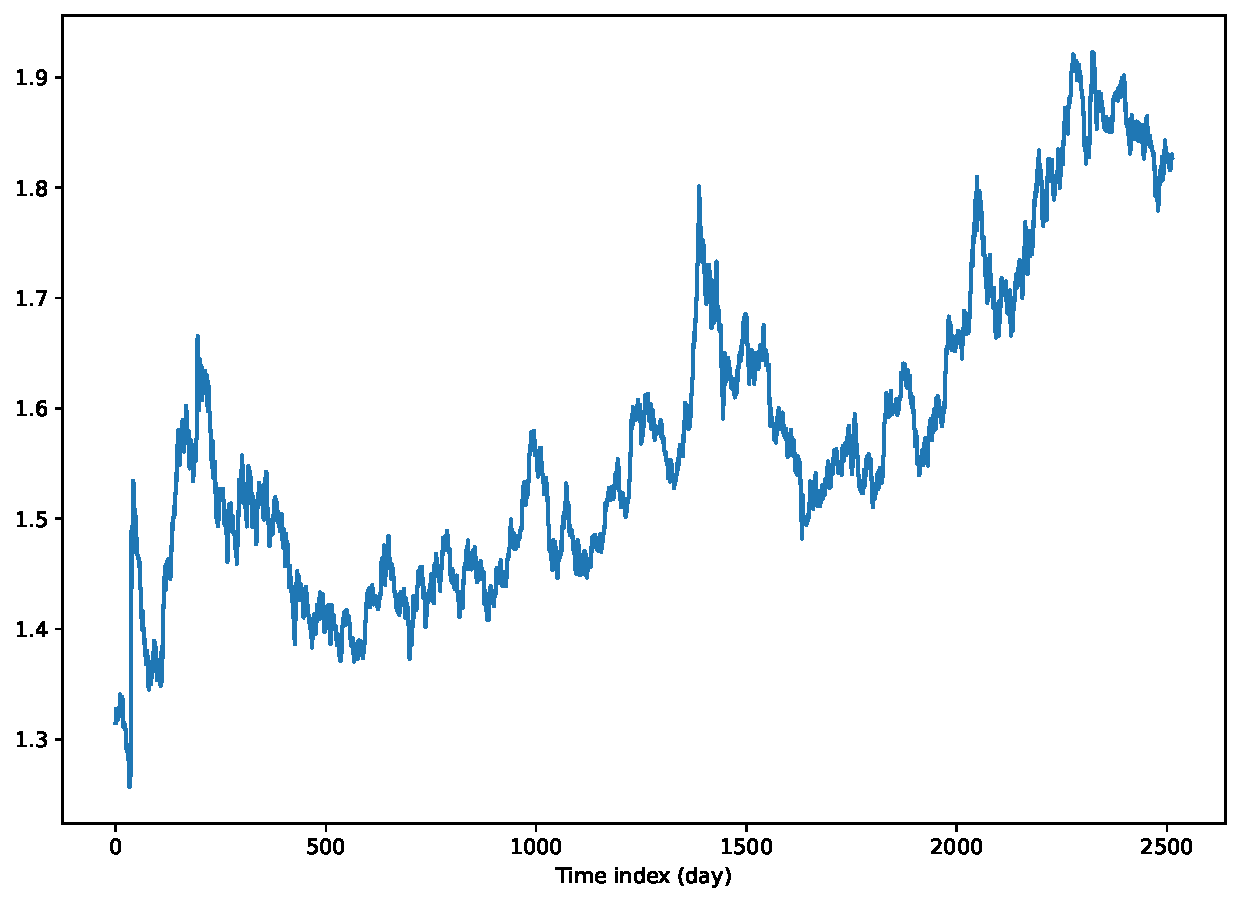
\includegraphics[width=\linewidth]{img/CHF_NZD.pdf}
    \caption{Exchange rate (close price) between Swiss franc and New Zealand dollar by day (2014-2024).}
    \label{fig:fx}
\end{figure}

%%%%%%%%%%%%%%%%%%%%%%%%%%%%%%%%%%%%%%%%%%%%%%%%%%%
\section{Methodology}
\label{sec.method}
%%%%%%%%%%%%%%%%%%%%%%%%%%%%%%%%%%%%%%%%%%%%%%%%%%%

% nói tổng quan ở đây, vẽ cái hình và bỏ vào
% Phương pháp của chúng tôi bao gồm hai phần chính hoạt động song song nhau: (1) - Feature extraction; (2) - Parameter synthesis. Tổng quan phương pháp được minh họa trong hình \ref{fig:flow}. Trong phần feature extraction, chúng tôi kết hợp hai loại đặc trưng từ mạng \verb|CNN| và \verb|LSTM|. Trong phần parameter synthesis, chúng tôi sử dụng \verb|MAML| để tổng hợp tham số của các mô hình. Với sự góp mặt của các đặc trưng \verb|LSTM| và \verb|CNN|, chúng tôi kỳ vọng sẽ rút trích được các đặc trưng ẩn trong dữ liệu aperiodic. Bằng việc sử dụng \verb|MAML| trong quá trình tổng hợp trọng số, phương pháp đề xuất được kỳ vọng là một giải pháp thay thế hợp lý và hiệu quả cho các mô hình ensemble truyền thống trong việc giảm thiểu tác động của sự biến thiên variance, tổng hợp hiệu quả các yếu tố ngoại lai, cũng như giữ được các hidden long-term dependency ẩn trong quá khứ.

Our method consists of two main parts that work in parallel: (1) - Feature extraction; (2) - Parameter synthesis. The overview of the method is illustrated in \ref{fig:flow}. In the feature extraction part, we combine two types of features from \verb|CNN| and \verb|LSTM| networks. In the parameter synthesis part, we use \verb|MAML| to synthesize the parameters of the models. Due to the contribution of \verb|LSTM| and \verb|CNN| features, we expect to effectively extract hidden features from aperiodic data. By using \verb|MAML| in the weight synthesis process, the proposed method is expected to be a reasonable and effective alternative to traditional ensemble models in minimizing the impact of variance variation, effectively synthesizing external factors, and preserving hidden long-term dependencies in the past.

\begin{figure*}[ht]
    \centering
    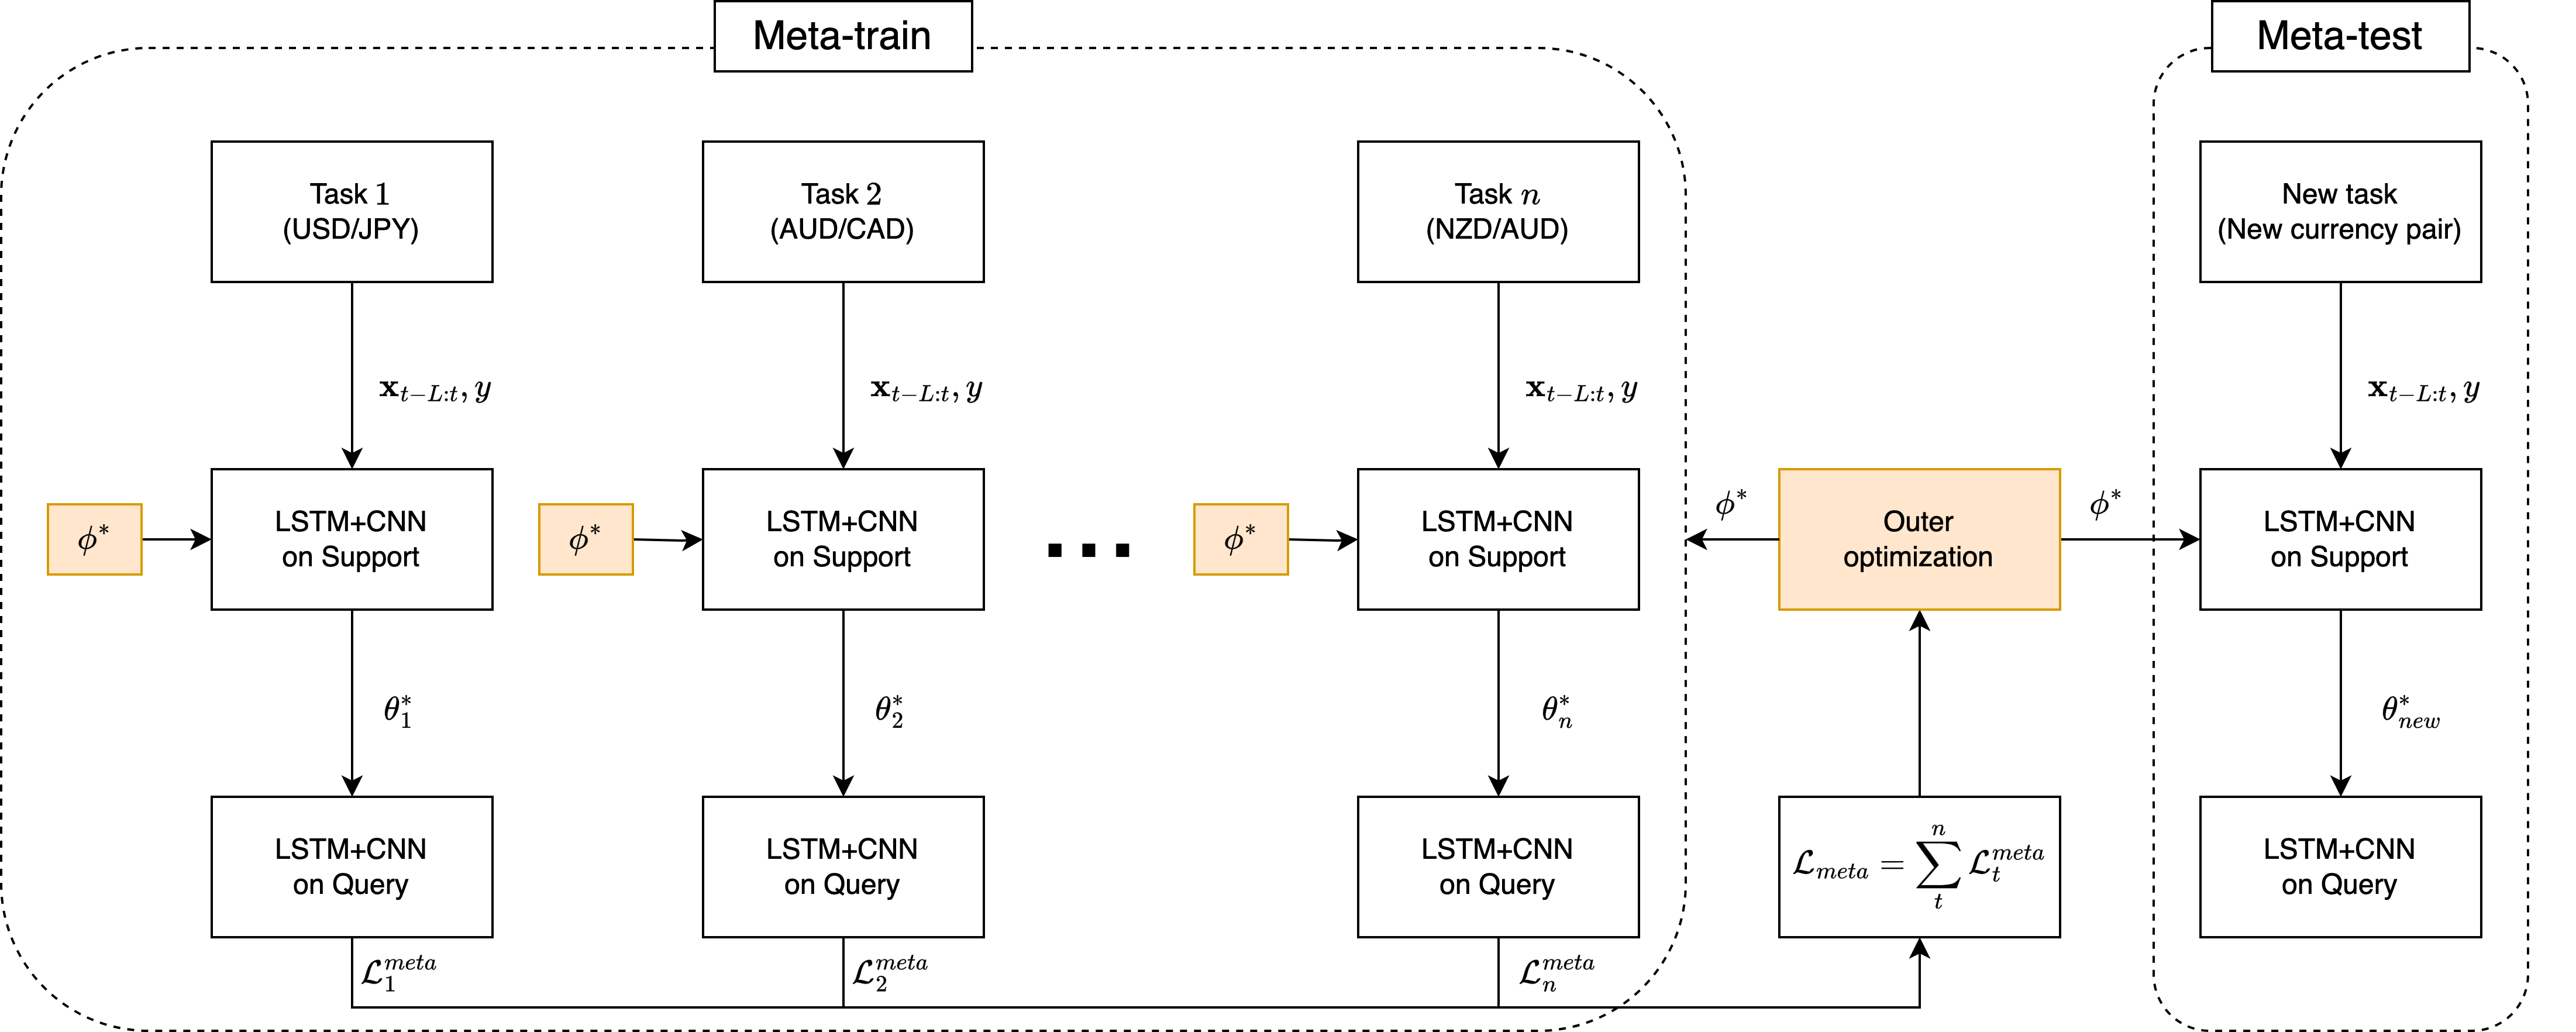
\includegraphics[width=\textwidth]{img/meta.png}
    \caption{The full-flow of meta-training and meta-testing on multi-fx data. Each currency pair is regarded as a task.}
    \label{fig:flow}
\end{figure*}

\subsection{Data preparation}

% Phương pháp đề xuất sử dụng các thuật toán ML để huấn luyện mô hình. Do đó, dữ liệu cần được tổ chức lại để các thuật toán ML có thể hoạt động được. Trong trường hợp dữ liệu bao gồm nhiều datasets khác nhau thuộc cùng một lĩnh vực, mỗi dataset sẽ được coi là một task của \verb|MAML|. Trong trường hợp dữ liệu bao gồm một dataset duy nhất, cần chia nhỏ dataset này thành các tập con ứng với các task riêng biệt. Tóm lại, tập dữ liệu sau khi chuẩn bị bao gồm $n$ tasks: $\mathcal{D} = \left\{ \mathcal{D}_t \right\}_{t=1}^{n}$. Dữ liệu tại mỗi task được chia thành tập support và query: $\mathcal{D}_t = \left\{ \mathcal{D}_t^{support}, \mathcal{D}_t^{query} \right\}$.

The proposed method uses ML algorithms to train the model. Therefore, the data needs to be reorganized so that the ML algorithms can work. In case the data includes many different datasets belonging to the same field, each dataset will be considered a task of \verb|MAML|. In case the data includes a single dataset, it is necessary to divide this dataset into subsets corresponding to separate tasks. In summary, the prepared dataset includes $n$ tasks: $\mathcal{D} = \left\{ \mathcal{D}_t \right\}_{t=1}^{n}$. The data at each task is divided into support and query sets: $\mathcal{D}_t = \left\{ \mathcal{D}_t^{support}, \mathcal{D}_t^{query} \right\}$.

\vspace{2mm}

% Một sample dữ liệu bao gồm các cặp giá trị $(\mathbf{x}_{t-L:t}, y)$. Trong đó, $\mathbf{x}_{t-L:t}$ bao gồm $L$ giá trị lịch sử tính từ thời điểm $t$ trở về trước; $y\in \{0,1\}$ là nhãn dữ liệu, thể hiện xu hướng giảm, hoặc tăng của mẫu dữ liệu $x_{t+1}$ so với $x_{t}$. Tùy vào từng bài toán và cách cài đặt mà các phần tử trong $\mathbf{x}_{t-L:t}$ có thể là các vector hoặc các scalar number. Ví dụ, đối với dữ liệu chứng khoán, $\mathbf{x}_{t-L:t}$ có thể chứa các vector dữ liệu $\vec x_i = (\text{open, low, high, close})$ hoặc chỉ một giá trị close price duy nhất.

A data sample consists of pairs of values $(\mathbf{x}_{t-L:t}, y)$. In which, $\mathbf{x}_{t-L:t}$ includes $L$ historical values from time $t$ back; $y\in \{0,1\}$ is the data label, showing the decreasing or increasing trend of the data sample $x_{t+1}$ compared to $x_{t}$. Depending on each problem and the implementation, the elements in $\mathbf{x}_{t-L:t}$ can be vectors or scalar numbers. For example, for stock data, $\mathbf{x}_{t-L:t}$ can contain $L$ data vectors $\vec x_i = (\text{open, low, high, close})$ or just a single close price value.

% nói từng cái, có thể sẽ vẽ hình cụ thể cho từng cái
% method phải chỉ ra được đoạn nào giải quyết thách thức nào (đã nêu ở intro)

% đến đoạn thực nghiệm thì sẽ mô tả sâu quá trình tìm kiếm tham số, quá trình chia dữ liệu, tải dữ liệu ở phụ lục
% nhận xét: nhấn mạnh vào việc giải quyết 3 thách thức nêu ở intro

\subsection{Feature extraction}

% Lấy cảm hứng từ nghiên cứu \cite{vo2017multi}, chúng tôi đề xuất kết hợp các đặc trưng rút trích được từ mạng \verb|LSTM| và \verb|CNN|. Cụ thể, chúng tôi đưa từng phần tử trong vector $\mathbf{x}_{t-L:t}$ qua một lớp \verb|MLP| có đầu ra lớn hơn số chiều của $\vec x_i, i\in[t-L, t]$ để phân giải thành các đặc trưng nhỏ $\vec x'_i$. Các đặc trưng này sau đó được truyền qua mạng \verb|LSTM| và \verb|CNN| để lần lượt rút trích các phụ thuộc thời gian dài hạn ($\mathbf{h}_{LSTM}$) và các đặc trưng thời gian cục bộ ($\mathbf{h}_{CNN}$). Để có thể khai thác tối đa các ràng buộc thời gian dài hạn, chúng tôi sử dụng \verb|BidirectionalLSTM| để rút trích từ hai phía của của $\mathbf{x}_{t-L:t}$. Toàn bộ quy trình rút trích đặc trưng được tóm tắt như sau:

Inspired by the \cite{vo2017multi} study, we propose to combine the features extracted from \verb|LSTM| and \verb|CNN| networks. Specifically, we pass each element in the vector $\mathbf{x}_{t-L:t}$ through a \verb|MLP| layer whose output'dimension is larger than the one of $\vec x_i, i\in[t-L, t]$ to decompose it into smaller features $\vec x'_i$. These features are then passed through \verb|LSTM| and \verb|CNN| networks to extract long-term temporal dependencies ($\mathbf{h}_{LSTM}$) and local temporal features ($\mathbf{h}_{CNN}$), respectively. To exploit the long-term temporal constraints, we use \verb|BidirectionalLSTM| to extract from both sides of $\mathbf{x}_{t-L:t}$. The entire feature extraction process is summarized as follows:

\begin{align}
    \mathbf{x'}_{t-L:t} &= \mathbf{FullyConnected}\left( \mathbf{x'}_{t-L:t} \right)\\
    \mathbf{h}_{LSTM} &= \mathbf{BidirectionalLSTM}\left( \mathbf{x'}_{t-L:t} \right)\\
    \mathbf{h}_{CNN} &= \mathbf{Convolution1D}\left( \mathbf{x'}_{t-L:t} \right)
    \label{eq:feature}
\end{align}

\vspace{2mm}

% Mạng \verb|LSTM| duy trì giá trị cell-state nhằm lưu trữ có chọn lọc các phụ thuộc dài hạn. Điều này rất thích hợp trong việc giải quyết các bài toán time-series data. Mặt khác, giá trị tương lai thường phụ thuộc rất lớn vào các giá trị lịch sử gần nhất. Chúng tôi đề xuất sử dụng mạng \verb|CNN| để nhấn mạnh các đặc trưng cục bộ, từ đó hướng một phần sự chú ý của mô hình vào các thời điểm nhất định. Do đó, phương pháp đề xuất không chỉ nhớ được các đặc trưng long-term mà còn highlight được các đặc trưng short-term.

The \verb|LSTM| network maintains cell-state values ​​to selectively store long-term dependencies. This is very suitable for solving time-series data problems. On the other hand, future values ​​often depend heavily on recent historical values. We propose to use the \verb|CNN| network to emphasize local features, thereby directing part of the model's attention to certain time points. Therefore, the proposed method can not only remember long-term features but also highlight short-term features.

\vspace{2mm}

% Tiếp đến, $\mathbf{h}_{LSTM}$ và $\mathbf{h}_{CNN}$ được nối với nhau (phương trình \ref{eq:concat}) sau đó chuyển đến phần phân lớp của mạng NN (phương trình \ref{eq:clf}).

Next, $\mathbf{h}_{LSTM}$ and $\mathbf{h}_{CNN}$ are concatenated (equation \ref{eq:concat}) and then passed to the classification part of the neural network (equation \ref{eq:clf}).

\begin{align}
    \mathbf{h}_{t-L:t} &= \mathbf{Concatenate}\left( \mathbf{h}_{LSTM}, \mathbf{h}_{CNN} \right) \label{eq:concat} \\
    \hat y &= \mathbf{FullyConnected}\left( \mathbf{h}_{t-L:t} \right) \label{eq:clf}
\end{align}

\subsection{Effective synthesis\\of models' parameters}

% Chúng tôi sử dụng \verb|MAML| để huấn luyện và tổng hợp trọng số của các mô hình tại các task. Như đã đề cập trong phần \ref{sec.relatedWork}, tối ưu tham số theo cách tiếp cận của ML chính là đi giải hai phương trình \ref{eq:inner_opt} và \ref{eq:outer_opt} bằng các phương pháp tối ưu trên dữ liệu support và query. Cụ thể, quá trình tối ưu bao gồm nhiều bước toàn cục (outer optimization), thực hiện trên tất cả các tasks tham gia huấn luyện. Mỗi bước toàn cục bao gồm nhiều bước cục bộ (inner optimization) thực hiện trên từng task riêng lẻ. Tại bước toàn cục $r$, quá trình tối ưu cục bộ lần thứ $e$ tại tập support của task $t$ diễn ra như sau:

We use \verb|MAML| to train and aggregate the weights of the models at the tasks. As mentioned in \ref{sec.relatedWork}, parameter optimization in the ML approach is to solve the two equations \ref{eq:inner_opt} and \ref{eq:outer_opt} using optimization methods on the support and query data. Specifically, the optimization process includes many global steps (outer optimization), performed on all tasks participating in training. Each global step includes many local steps (inner optimization) performed on each individual task. At global step $r$, the $e$th local optimization process at the support set of task $t$ occurs as follows:

\begin{align}
    \begin{cases}
        \theta_t^{(0)} &= \phi_{r-1} \\
        \theta_t^{(e)} &= \theta_t^{(e-1)} - \alpha \nabla_{\theta} \mathcal{L}^{task}_t\left( \theta_t^{(e-1)}, \mathcal{D}_t^{support} \right)
    \end{cases}
\end{align} In which, $\phi_{r-1}$ is the result of the $r-1$ global optimization process, $\alpha$ is the inner learning rate.

\vspace{2mm}

% Tiếp đó, quá trình outer optimization tại bước toàn cục được thực hiện bằng cách tổng hợp độ lỗi trên tập query của các task và tối ưu trên đó (phương trình \ref{eq:outer_sol}).

Next, the outer optimization process at the global step is performed by aggregating the losses on the query set of the tasks and optimizing on it (equation \ref{eq:outer_sol}).

\begin{align}
    \begin{cases}
        \phi_0 = \text{Random Initialization}\\
        \phi_r = \phi_{r-1} - \beta \nabla_{\phi} \sum_{t=1}^n{\mathcal{L}^{meta}_t \left( \theta_t^*(\phi), \mathcal{D}_t^{query} \right)}
    \end{cases}
    \label{eq:outer_sol}
\end{align} Where, $\beta$ is the outer learning rate.

% Giả sử thuật toán chạy $E$ steps trong inner optimization, lượng đạo hàm tại phương trình \ref{eq:outer_sol} được viết lại như sau (the notations of dataset are removed):

Assuming the algorithm runs $E$ steps in inner optimization, the derivative quantity at equation \ref{eq:outer_sol} is rewritten as follows (the notations of dataset are removed):

\begin{align*}
    &\beta \nabla_{\phi} \sum_{t=1}^n{\mathcal{L}^{meta}_t \left( \theta_t - \alpha \nabla_{\theta} \mathcal{L}^{task}_t\left( \theta_t \right) \right)}\\
    = &\beta \sum_{t=1}^n{ \frac{\partial \mathcal{L}^{meta}_t\left(\theta_t^{(E)}\right)}{\partial \theta_t^{(E)}} \frac{\partial \theta_t^{(E)}}{\partial \phi}}\\
    = &\beta \sum_{t=1}^n{ \nabla_{\theta} \mathcal{L}^{meta}_t\left(\theta_t^{(E)}\right) \prod_{j=0}^{E-1} {\left[\mathbb{I} - \alpha\nabla^2_{\theta}\mathcal{L}^{task}_{t}\left(\theta_t^{(j)}\right)\right]}} \numberthis
    \label{eq:outer_sol_}
\end{align*}

% Sự xuất hiện của tích các đạo hàm bậc hai trong phương trình \ref{eq:outer_sol_} khiến quá trình đạo hàm trở nên phức tạp vì phải tốn rất nhiều chi phí để duy trì các ma trận Hessian. Do đó, số bước tính toán để tìm ra $\theta^*$ cần phải hạn chế. Trên thực tế, các phương pháp sử dụng ML \citep{fallah2020personalized, chen2018federated, nguyen2022meta,finn2017model, li2017meta} thường sẽ chọn $E\in [1,5]$.

The presence of the product of second order derivatives in the equation \ref{eq:outer_sol_} makes the derivation process complicated because it requires a lot of overhead to maintain the Hessian matrices. Therefore, the number of computational steps to find $\theta^*$ needs to be limited. In practice, methods using ML \citep{fallah2020personalized, chen2018federated, nguyen2022meta,finn2017model, li2017meta} often choose $E\in [1,5]$.

%%%%%%%%%%%%%%%%%%%%%%%%%%%%%%%%%%%%%%%%%
\section{Numerical experiment}
\label{sec.experiment}
%%%%%%%%%%%%%%%%%%%%%%%%%%%%%%%%%%%e%%%%%%

\subsection{Dataset \& Metric}

% FX nói riêng và các chỉ số tài chính nói chung là dạng dữ liệu điển hình cho aperiodic time-series data. Do đó, chúng tôi chọn loại dữ liệu này để kiểm thử mô hình. Cụ thể, chúng tôi cấu hình hai bộ dữ liệu sử dụng dữ liệu FX. Bộ dữ liệu \verb|USD/JPY| chỉ gồm dữ liệu của cặp tiền tệ USD/JPY, được chia thành 60 tập dữ liệu con theo trình tự thời gian với kích thước bằng nhau. Dữ liệu được sample theo giờ từ năm 2000 đến năm 2024, bao gồm các thuộc tính open, low, high, và close price. Bộ dữ liệu \verb|multi-fx| bao gồm 60 cặp tiền tệ giữa 18 quốc gia Australia, Canada, Switzerland, Denmark, EU, United Kingdom, Hong Kong, Iceland, Japan, Norway, New Zealand, Singapore, Sweden, Turkey, United States, Mexico, China, South Africa. Dữ liệu có thuộc tính tương tự như \verb|USD/JPY| và được sample theo ngày từ năm 2014 đến 2024. Số lượng mẫu dữ liệu của hai tập dữ liệu là tương đương nhau và xấp xỉ $156000$ mẫu.

FX in particular and financial indices in general are typical data types for aperiodic time-series data. Therefore, we choose this type of data to test the model. Specifically, we configure two datasets using FX data. The \verb|USD/JPY| dataset consists of only data of the USD/JPY currency pair, divided into 60 time-sequenced subsets of equal size. The data is sampled hourly from 2000 to 2024, including the attributes of open, low, high, and close price. The \verb|multi-fx| dataset consists of 60 currency pairs made up of 18 countries: Australia, Canada, Switzerland, Denmark, EU, United Kingdom, Hong Kong, Iceland, Japan, Norway, New Zealand, Singapore, Sweden, Turkey, United States, Mexico, China, South Africa. The data has similar attributes to \verb|USD/JPY| and sampled daily from 2014 to 2024. The number of data samples of these two datasets are similar and approximately $156000$ samples.

\vspace{2mm}

% Bộ dữ liệu \verb|multi-fx| được sử dụng để rút trích và tổng hợp thông tin về các yếu tố ngoại lai (i.e. thông tin thị trường, kinh tế, chính trị,...), vốn được cho là có ảnh hưởng đến kết quả của một chỉ số tài chính nhất định \citep{overreactioncontrarian,fama1970efficient,mech1993portfolio}. Bộ dữ liệu \verb|USD/JPY| được sử dụng để kiếm chứng giả thuyết của chúng tôi về việc dữ liệu tương lai ngầm phụ thuộc vào các thời điểm nhất định trong quá khứ và cần phải tổng hợp đặc trưng quá khứ một cách hiệu quả để làm rõ được các phụ thuộc này.

The \verb|multi-fx| dataset is used to extract and aggregate information about outliers (i.e. market, economic, political, etc.) that are believed to influence the outcome of a given financial index \citep{overreactioncontrarian,fama1970efficient,mech1993portfolio}. The \verb|USD/JPY| dataset is used to test our hypothesis that future data implicitly depend on certain points in the past and that efficient past feature aggregation is needed to reveal these dependencies.

\vspace{2mm}

% Nghiên cứu sử dụng macro accuracy, macro precision, macro recall, và macro F1 để đánh giá các mô hình. Theo đó, trong quá trình inference, mô hình sẽ chạy trên từng task để tính metrics của mỗi task. Sau đó tính trung bình cộng các metrics của các task để thu được kết quả cuối.

The study uses macro accuracy, macro precision, macro recall, and macro F1 score to evaluate the models. Accordingly, during the inference phase, the model will run on each task to calculate the metrics of each task. Then, the average of the metrics of the tasks is calculated to obtain the final result.

\vspace{2mm}
\subsection{Experiment}

% Chúng tôi tiến hành so sánh phương pháp đề xuất với mô hình \verb|NHITS| thông qua các metrics nêu trên. Dữ liệu tổng quan được cấu trúc thành training sets, validation sets, và testing sets với tỷ lệ 6:2:2. Tập train dùng để huấn luyện mô hình, tập validation dùng để tìm kiếm siêu tham số và tập test để đánh giá mô hình. Đối với \verb|NHITS|, chúng tôi chia dữ liệu như bình thường theo tỷ lệ định sẵn ở trên. Đối với thuật toán đề xuất, vì quá trình meta-training và meta-testing đòi hỏi phải chia dữ liệu thành các task nhỏ, và cho phép mô hình adapt trên tập support của mỗi task, chúng tôi chia dữ liệu thành 60 tasks. Trong mỗi task, tập support chiếm 20\% với mục đích để mô hình học cách thích ứng với dữ liệu, tập query chiếm 80\% để kiểm tra khả năng tương thích của mô hình. Chúng tôi sử dụng 30 tasks để meta-train, 15 tasks để meta-validate, 15 tasks để meta-test. Với cách chia này, chúng tôi đảm bảo được tính công bằng khi mô hình ML được huấn luyện với lượng dữ liệu tương đương mô hình \verb|NHITS|.

We compare the proposed method with \verb|NHITS| using the above metrics on \verb|USD/JPY| and \verb|multi-fx| datasets. We also test different feature extractors (\verb|LSTM|, \verb|CNN|) for the proposed method to demonstrate the deep data understanding capabilities of \verb|LSTM+CNN|. The overall data is structured into training sets, validation sets, and testing sets with a ratio of 6:2:2 for training, fine-tuning and testing model, respectively.

\vspace{2mm}

For \verb|NHITS| model, we split the data as usual according to the above predetermined ratio. For the proposed algorithm, because the meta-training and meta-testing processes require dividing the data into small tasks, and allowing the model to adapt on the support set of each task, we split the data into 60 tasks (see table \ref{tab:stat_} for statistical detail). In each task, the support set accounts for 20\% with the purpose of letting the model adapt to the data, the query set accounts for 80\% to check the model's compatibility. We use 30 tasks for meta-training, 15 tasks for meta-validation, and 15 tasks for meta-testing. With this division, we ensure the fairness that the ML model is trained with the same amount of data as \verb|NHITS|. After the data configuration, we perform experiment as in appendix \ref{app:our_experiment} and \ref{app:nhits_experiment}.

\begin{table}
    \centering
    \caption{Statistics on USD/JPY and multi-fx.}
    \label{tab:stat_}
    \begin{tabular}{ccccccc}
    \toprule
    \multirow{2}{*}{Dataset} & \multirow{2}{*}{\#task} & \multirow{2}{*}{\#samples} & \multicolumn{4}{c}{\#samples/task}  \\
    \cline{4-7}
                             &                         &                            & min & mean  & std   & max             \\
    \hline
    \Verb|USD/JPY|           & 60                      & 150,175                     & 2,502 & 2,502.92 & 0.28 & 2,503           \\
    \Verb|multi-fx|          & 60                      & 154,440                     & 2,467 & 2,575 & 58.61   & 2748           \\
    \bottomrule
    \end{tabular}
\end{table}

%%%%%%%%%%%%%%%%%%%%%%%%%%%%%%%%%%%%%%%%%%%%%%%%
\section{Result \& Discussion}
\label{sec.results}
%%%%%%%%%%%%%%%%%%%%%%%%%%%%%%%%%%%%%%%%%%%%%%%%

% nói 1 chút về việc xài lstm+cnn/meta-learning sẽ giảm sự phụ thuộc của kết quả vào mạng NN/siêu tham số
% cụ thể, khi xài ML, tham số finetune rất dễ, cái nào cũng cao, chỉ cần chọn ra cái cao nhất
% giải thích tại sao cnn perform poorly: quá chú ý đến đặc trưng cục bộ mà quên mất các phụ thuộc dài hạn

% Bảng \ref{tab:rs} so sánh kết quả giữa mô hình đề xuất và mô hình \verb|NHITS| trên các tập dữ liệu kể trên. Phương pháp của chúng tôi đạt mức hội tụ cao hơn hẳn so với mô hình \verb|NHITS| thể hiện trên tất cả các metrics. Cụ thể, độ chính xác cải thiện từ 5\% đến 11\% so với \verb|NHITS| trên dữ liệu \verb|USD/JPY| và \verb|multi-fx|. Các metrics còn lại cũng đều tăng từ 5\% đến 20\%. Sau đây, chúng tôi phân tích kết quả này dựa trên hai yếu tố: (1) - Khả năng rút trích đặc trưng; (2) - Khả năng tổng hợp mô hình.

Table \ref{tab:rs} compares the results between the proposed model and the \verb|NHITS| model on the above datasets. Our method achieves a much higher convergence rate than the \verb|NHITS| model on all metrics. Specifically, the accuracy improves from 5\% to 11\% compared to \verb|NHITS| on \verb|USD/JPY| and \verb|multi-fx| data. The remaining metrics also increase from 5\% to 20\%. Next, we analyze this result based on two factors: (1) - Feature extraction ability; (2) - Model synthesis ability.

\vspace{2mm}

\begin{table*}
    \centering
    \caption{Classification results (\%) of NHITS and our method using USD/JPY and multi-fx datasets. Best results per metrics are boldfaced.}
    \label{tab:rs}
    \begin{tabular}{c|c|cccc}
    \toprule
    \multicolumn{1}{c}{}                          &                                    & $accuracy$            & $precision$           & $recall$              & $F1$                    \\
    \hline
    \multirow{3}{*}{\Verb|USD/JPY|}  & \Verb|NHITS|          & 53.29                 & 52.38                 & 52.23                 & 51.87                   \\
                                                & Ours(\Verb|LSTM|)     & $57.12±0.08$ & $58.32±2.72$ & $57.44±2.62$ & $56.87±3.56$    \\
                                                & Ours(\Verb|LSTM+CNN|) & $\mathbf{58.05±0.01}$ & $\mathbf{59.57±2.53}$ & $\mathbf{58.31±2.57}$ & $\mathbf{56.6±3.74}$    \\
    \hline
    \multirow{3}{*}{\Verb|multi-fx|} & \Verb|NHITS|          & 51.12                 & 51.22                 & 51.16                 & 50.54                   \\
                                                & Ours(\Verb|LSTM|)     & $61.23±0.06$          & $70.52±9.17$          & $69.51±9.31$          & $68.9±10.0$             \\
                                                & Ours(\Verb|LSTM+CNN|) & $\mathbf{62.39±0.06}$ & $\mathbf{71.11±9.34}$ & $\mathbf{70.14±9.6}$  & $\mathbf{69.21±11.07}$  \\
    \bottomrule
    \end{tabular}
\end{table*}

\subsection{Feature extraction ability}

% Chúng tôi huấn luyện ba mô hình \verb|CNN|, \verb|LSTM|, \verb|LSTM+CNN| trên 2600 mẫu dữ liệu \verb|CHF/NZD| theo cách thông thường. Sau khi quan sát quá trình huấn luyện của chúng (hình \ref{fig:lstm_cnn}), chúng tôi nhận thấy khả năng rút đặc trưng cục bộ tuyệt vời trên dữ liệu ngắn hạn của \verb|CNN|. Mặt khác, \verb|LSTM| không cải thiện sau 40 epochs, chứng tỏ rằng nếu chỉ tập trung vào khai thác các phụ thuộc ngắn/dài hạn mà không rút trích đặc trưng đủ sâu thì sẽ không mang lại kết quả cao. Khi kết hợp cả hai đặc trưng, mô hình cho thấy sự cải thiện trong khả năng học trên tập train. Mức hội tụ nhìn chung đều tăng so với việc sử dụng từng mô hình riêng lẻ. Điều này có thể được lý giải thông qua việc \verb|LSTM| đã tích hợp thành công các long-term feature vào mô hình, cũng như việc tận dụng các đặc trưng cục bộ của \verb|CNN|.

We trained three models \verb|CNN|, \verb|LSTM|, \verb|LSTM+CNN| on 2600 samples of \verb|CHF/NZD| data in the conventional way. After observing their training process (figure \ref{fig:lstm_cnn}), we found that \verb|CNN| has excellent local feature extraction ability on short-term data. On the other hand, \verb|LSTM| does not improve after 40 epochs, indicating that focusing on exploiting short/long-term dependencies without extracting deep enough features will not yield good results. When combining both features, the model shows an improvement in learning ability on the training set. The convergence rate is generally higher than when using each model separately. This can be explained by the fact that \verb|LSTM| successfully integrated long-term features into the model, as well as taking advantage of the local features of \verb|CNN|.

\begin{figure}
    \centering
    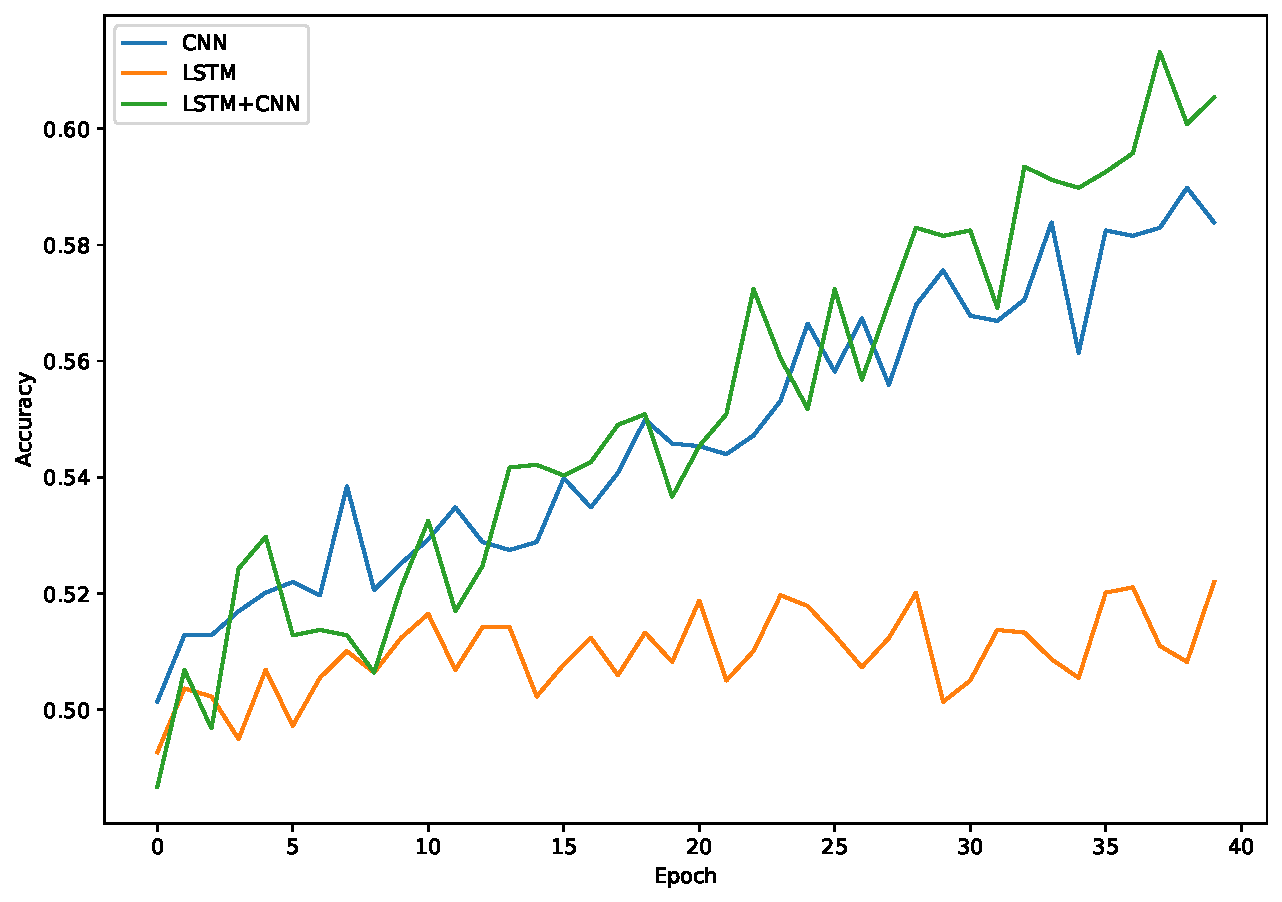
\includegraphics[width=\linewidth]{img/models.pdf}
    \caption{Training process of LSTM, CNN, and LSTM+CNN using 2600 samples from CHF/NZD dataset.}
    \label{fig:lstm_cnn}
\end{figure}

\vspace{2mm}

% Tuy nhiên, khi quan sát kết quả trên tập validation, cả ba mô hình trên không đều cho kết quả rất tệ. Lý giải cho điều này, chúng tôi nhận định rằng dù có thể học tốt trên tập train nhưng các mô hình đều mất đi tính tổng quát hóa vì đây là loại dữ liệu phức tạp, khác với các dữ liệu như hình ảnh, video, hoặc dữ liệu có chu kỳ. Nếu khả năng thích ứng của mô hình không cao, kết quả tệ trên tập validation là điều có thể lường trước được. Mặc dù vậy, \textbf{đồ thị trong hình \ref{fig:lstm_cnn} cho thấy chúng ta không thể phủ nhận khả năng rút trích đặc trưng của} \verb|LSTM+CNN|.

However, when observing the results on the validation set, all three models above give very poor results. To explain this, we think that although they can learn well on the training set, the models lose their generalization ability because this is a complex type of data, different from data such as images, videos, or periodic data. If the model's adaptability is not high, poor results on the validation set are predictable. However, \textbf{the graph in figure \ref{fig:lstm_cnn} shows that we cannot deny the feature extraction ability of} \verb|LSTM+CNN|.

\vspace{2mm}

% Sau này, khi sử dụng thuật toán ML để huấn luyện các mạng rút trích đặc trưng, chúng tôi còn nhận thấy mô hình sử dụng đặc trưng kết hợp ít bị phụ thuộc vào learning rate hơn các mô hình sử dụng đặc trưng đơn lẻ. Cụ thể, đối với không gian learning rate mà chúng tôi định nghĩa trong Appendix \ref{app:lr}, tất cả các mô hình đều hội tụ với độ chính xác thấp nhất từ 54\%. Việc này minh chứng cho khả năng ưu việt của đặc trưng do \verb|LSTM+CNN| mang lại.

Later, when we used ML algorithms to train feature extraction networks, we also found that the model using combined features was less dependent on the learning rate than the model using single features. Specifically, for the learning rate space we defined in Appendix \ref{app:lr}, all models converged with an accuracy of at least 54\%. This demonstrates the superiority of the feature provided by \verb|LSTM+CNN|.

\begin{figure}
    \centering
    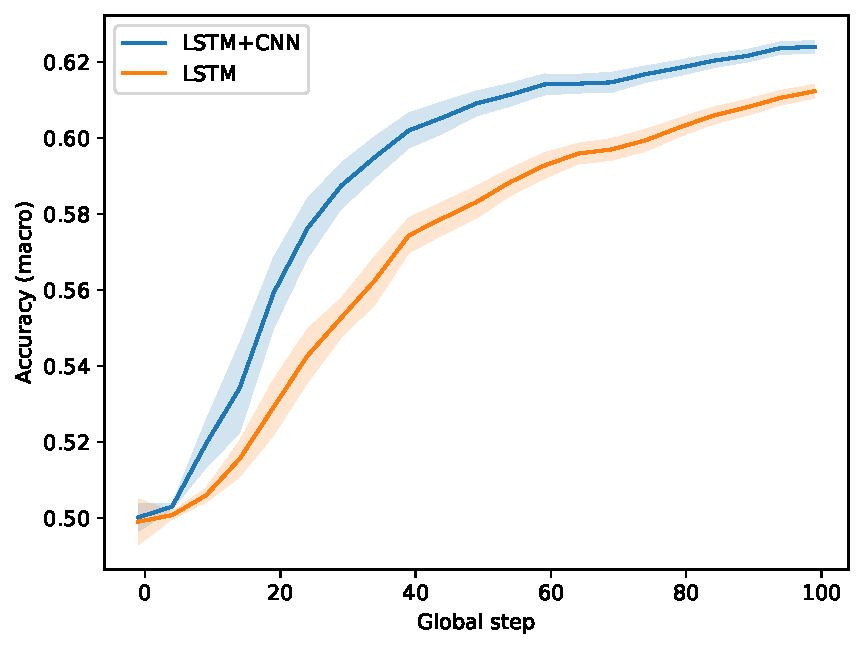
\includegraphics[width=\linewidth]{img/acc.pdf}
    \caption{Convergence process on validation set of neural network using LSTM+CNN feature and LSTM feature only (multi-fx dataset). The blur domains cover 99.73\% ($±3\sigma$) values of accuracies.}
    \label{fig:lstm_cnn_feature}
\end{figure}

% Quan sát quá trình rút trích đặc trưng của \verb|NHITS|, có thể thấy mô hình này đang cố gắng mô phỏng lại quá trình phân giải tần số của Fourier transform. Tuy nhiên, trong toàn bộ quá trình thực thi, \verb|NHITS| sử dụng các kiến trúc rất đơn giản (chỉ bao gồm các lớp \verb|MLP| và \verb|Pooling|). Đối với các dữ liệu phức tạp và phi chu kỳ, sử dụng các layer \verb|MLP| là không đủ để rút trích các đặc trưng ẩn.

Looking at the feature extraction process of \verb|NHITS|, it can be seen that this model tries to simulate the frequency resolution process of Fourier transform. However, in the whole implementation, \verb|NHITS| uses a very simple architecture (only including \verb|MLP| and \verb|Pooling| layers). For complex and non-periodic data, using \verb|MLP| layers is not enough to extract hidden features.

\subsection{Sub-model synthesis ability}

% Lý do phương pháp huấn luyện thông thường không đạt hiệu quả cao mặc cho khả năng rút trích đặc trưng đã được cải thiện là vì thiếu khả năng sử dụng đặc trưng một cách hiệu quả. Khả năng này trong các nghiên cứu trước đây thường được cải thiện bằng việc sử dụng các mô hình ensemble. Chúng tôi đã thử sử dụng các mô hình truyền thống (boosting, stacking) nhằm tăng độ chính xác của mô hình nhưng sớm nhận ra rằng phương pháp này không khả thi. Ngay cả khi chúng tôi vét cạn cạn trên không gian hyper-parameter để tìm ra kiến trúc mô hình con tốt nhất bằng \verb|AutoKeras| \cite{jin2023autokeras}, độ chính xác thu được trên tập \verb|USD/JPY| chỉ ở mức 52.53\% và 53.71\%, respectively.

The reason why conventional training methods do not perform well despite the improved feature extraction capabilities is the lack of the ability to use features effectively. This ability in previous studies has often been improved by using ensemble models. We tried using traditional models (boosting, stacking) to increase the model accuracy but soon realized that this method was not feasible. Even when we performed brute-force search the hyper-parameter space to find the best sub-model architecture using \verb|AutoKeras| \cite{jin2023autokeras}, the accuracy on \verb|USD/JPY| was only 52.53\% and 53.71\%, respectively.

\vspace{2mm}

% Khi sử dụng \verb|MAML| để tổng hợp đặc trưng của mô hình \verb|LSTM| và \verb|LSTM+CNN|, khả năng tương thích (thể hiện qua việc hội tụ sớm) cũng như kết quả (thể hiện qua độ chính xác) của mô hình sử dụng \verb|LSTM+CNN| cao hơn hoàn toàn so với mô hình chỉ sử dụng \verb|LSTM| (xem hình \ref{fig:lstm_cnn_feature}). Thật vậy, chỉ sau 40 epochs, các đặc trưng \verb|LSTM+CNN| cho mức hội tụ trên 60\% và sau 100 epochs, mô hình hội tụ ở mức 62\%, vượt trên những gì các đặc trưng \verb|LSTM| có thể làm được. Độ biến thiên của các giá trị accuracy là rất nhỏ, cho thấy sự ổn định của \verb|MAML|. Đối với mô hình ML chỉ sử dụng \verb|CNN|, độ chính xác cũng như giá trị lỗi thậm chí còn không cải thiện trong toàn bộ quá trình huấn luyện. Giải thích cho việc này, chúng tôi cho rằng các đặc trưng của \verb|CNN| đã quá tập trung vào tính cục bộ của dữ liệu mà bỏ qua các phụ thuộc dài hạn, vốn là một đặc trưng quan trọng của dữ liệu time-series. Trái lại, đặc trưng của \verb|LSTM+CNN| không chỉ nắm bắt được các phụ thuộc dài hạn mà còn có thể highlight các tính chất cục bộ trong dữ liệu, khiến cho nó hoàn toàn outperform \verb|CNN| cũng như \verb|NHITS|. Do đó, \textbf{chúng tôi kết luận rằng ML tỏ ra linh hoạt và đạt hiệu quả cao trong việc tổng hợp các sub-model so với các mô hình ensemble cứng nhắc truyền thống}.

When using \verb|MAML| to synthesize the features of the \verb|LSTM| and \verb|LSTM+CNN| models, the compatibility (indicated by early convergence) as well as the results (indicated by accuracy) of the model using \verb|LSTM+CNN| are significantly higher than those of the model using only \verb|LSTM| (see figure \ref{fig:lstm_cnn_feature}) and the \verb|NHITS| model. Indeed, after only 40 epochs, the \verb|LSTM+CNN| features converge to over 60\% and after 100 epochs, the model converges to 62\%, exceeding what the \verb|LSTM| features can do. The variation of the accuracy values ​​is very small, indicating the stability of \verb|MAML|. For the ML model using only \verb|CNN|, the accuracy and error values ​​do not even improve during the entire training process. We explain this by saying that the features of \verb|CNN| focus too much on the locality of the data and ignore the long-term dependencies, which is an important feature of time-series data. In contrast, the features of \verb|LSTM+CNN| not only capture the long-term dependencies but also highlight the local properties in the data, making it completely outperform \verb|CNN| as well as \verb|NHITS|. Therefore, \textbf{we conclude that ML is more flexible and efficient in synthesizing sub-models than traditional rigid ensemble models}.

\vspace{2mm}

% Khi tiếp cận dữ liệu \verb|USD/JPY| bằng ML, mô hình cũng cho độ chính xác cao. Bằng việc nhìn vào các khoảng thời gian trong quá khứ, \textbf{phương pháp đề xuất đã tỏ ra hiệu quả hơn trong việc nắm bắt các hidden long-term dependency thông qua việc tổng hợp hiệu quả các đặc trưng mà} \verb|LSTM| \textbf{dễ dàng quên đi trong quá trình huấn luyện}. Điều này đã chứng minh giả thuyết về sự tồn tại của các hidden long-term dependency mà chúng tôi nêu ra ở phần \ref{sec.intro}.

When approaching the \verb|USD/JPY| data using ML, the model also shows high accuracy. By looking at the past time periods, \textbf{the proposed method has proven to be more effective in capturing hidden long-term dependencies through the efficient aggregation of features that the} \verb|LSTM| \textbf{easily forgets during training}. This proves the hypothesis of the existence of hidden long-term dependencies that we stated in section \ref{sec.intro}.

% dis NHITS vì tổng hợp đặc trưng chỉ bằng phép cộng :v
% Trong quá trình tổng hợp các đặc trưng để đưa ra dự đoán cuối, \verb|NHITS| chỉ sử dụng các phép cộng trừ đơn giản. Điều này đặt trong ngữ cảnh của việc tổng hợp thông tin dựa trên các hàm nội suy và phần dư của input là hợp lý. Tuy nhiên, đối diện với sự phức tạp trong dữ liệu đòi hỏi một cấu trúc phức tạp hơn để có thể tổng hợp các đặc trưng một cách hợp lý hơn. Việc sử dụng nội suy trên dữ liệu có thể coi là rất đơn giản so với quá trình meta-optimization của các thuật toán ML. Hơn nữa, việc phân tách và kết hợp các dải tần số dữ liệu của \verb|NHITS| chỉ có thể hoạt động tốt nếu dữ liệu thực sự tồn tại chu kỳ. Dữ liệu phi chi kỳ như FX hoặc stock price có thể là điểm yếu chí mạng cho hướng tiếp cận này.

In the process of synthesizing features to make the final prediction, \verb|NHITS| only uses simple addition and subtraction. This is reasonable in the context of synthesizing information based on interpolation functions and input residuals and trying to simulate the synthesis of frequency bands. However, facing complexity in data requires a more complex structure to be able to synthesize features in a more reasonable way. Using interpolation on the data can be considered very simple compared to the meta-optimization process of ML algorithms. Furthermore, \verb|NHITS|'s separation and combination of data frequency bands can only work well if the data is truly periodic. Non-periodic data such as FX or stock prices can be a fatal weakness for this approach.

%%%%%%%%%%%%%%%%%%%%%%%%%%%%%%%%%%%%%%%%%
\section{Conclusion \& Future direction}
\label{sec.conc}
%%%%%%%%%%%%%%%%%%%%%%%%%%%%%%%%%%%%%%%%%

% Các bài toán trên aperiodic time-series data đặt ra một thử thách lớn cho các mô hình học máy hiện nay bởi tính bất định trong variance cũng như tính phi chu kỳ loại dữ liệu này. Bằng việc kết hợp các đặc trưng cục bộ và các phụ thuộc dài hạn cũng như khai thác các phụ thuộc ẩn trong từng khoảng thời gian quá khứ, chúng tôi đã cải khả năng của mô hình học máy trên các classification metrics trong bài toán dự đoán xu hướng giá của ngày tiếp theo trên dữ liệu FX. Thuật toán đề xuất đã chứng minh được khả năng vượt trội của mình khi so sánh với mô hình \verb|NHITS|.

Problems on aperiodic time-series data pose a great challenge to current machine learning models due to the uncertainty in variance as well as the aperiodicity of this type of data. By combining local features and long-term dependencies as well as exploiting hidden dependencies in each past time period, we have improved the ability of machine learning models on classification metrics in the problem of predicting the next day's price trend on FX data. The proposed algorithm has demonstrated its superior ability when compared with the \verb|NHITS| model.

\vspace{2mm}

% Trong tương lai, chúng tôi đề xuất hai hướng phát triển chính liên quan đến kiến trúc và tính cá nhân hóa của mô hình học.

In the future, we propose two main directions of development related to the architecture and personalization of the learning model.

\vspace{2mm}

% \textbf{Model architecture}. Phương pháp của chúng tôi được phát triển dưới dạng module với hai module chính hoạt động song song: Module rút trích đặc trưng và Module tổng hợp mô hình. Điều này cung chấp cho phương pháp của chúng tôi một khả năng nâng cấp linh hoạt. Thí nghiệm của chúng tôi chỉ minh họa một trường hợp điển hình trong việc rút trích và tổng hợp hiệu quả các đặc trưng. Bằng việc thay thế các mô hình rút trích đặc trưng khác nhau và sử dụng các thuật toán ML khác nhau, hoàn toàn có thể tạo ra mô hình mới với độ chính xác cao hơn.

\textbf{Model architecture}. Our method is modularized with two main modules operating in parallel: Feature Extraction Module and Model Synthesis Module. This provides our method with flexible scalability. Our experiment only illustrates a typical case of efficient feature extraction and synthesis. By replacing different feature extraction models and using different ML algorithms (\verb|Meta-SGD| \cite{li2017meta}, \verb|Reptile| \cite{nichol2018first}, \verb|iMAML| \cite{rajeswaran2019meta}), it is possible to create new models with higher accuracy.

\vspace{2mm}

% \textbf{Long-horizon problem}. Hoàn toàn có thể mở rộng phương pháp này để giải các bài toán về long-horizon prediction. Thật vậy, bằng việc thay đổi đầu ra và độ lỗi của mô hình, có thể tiến hành giải các bài toán này. Tuy nhiên, kiến trúc của các sub-model cần được nghiên cứu lại để phù hợp hơn với bài toán mới.

\textbf{Long-horizon problem}. It is possible to extend this method to solve long-horizon prediction problems. Indeed, by changing the output and error of the model, it is possible to solve these problems. However, the architecture of the sub-models needs to be re-examined to better suit the new problem.

% cite Meta-SGD, và 1 đống ML method vào đây để kiểu *ML có nhiều phương pháp, cần chạy thực nghiệm nhiều hơn
% cite iMAML, Reptile vào đây để làm future direction kiểu tối ưu lại ML vì chi phí hơi đắt
% apply các kỹ thuật cá nhân hóa để giảm thiểu variance trong kq vì variance hơi cao

%%%%%%%%%%%%%%%%%%%%%%%%%%%%%%%%%%%%%%%%%
\section{Acknowledgements}
%%%%%%%%%%%%%%%%%%%%%%%%%%%%%%%%%%%%%%%%%
% The work was carried out within the state assignment of Ministry of Science and Higher Education of the Russian Federation (No. AAAA-A18-118020190095-4, topic ``Quantum''). G.I.P is grateful for financial supports from JST SPRING, Grant Number JPMJSP2102. K. H. is grateful for financial support from MEXT-KAKENHI (JP19K05029, JP21K03400, JP21H01998, and JP22H02170). R.M. is grateful for financial supports from MEXT-KAKENHI (22H05146, 21K03400 and 19H04692).

%%%%%%%%%%%%%%%%%%%%%%%%%%%%%%%%%%%%%%%%%
\section{Author contributions}
%%%%%%%%%%%%%%%%%%%%%%%%%%%%%%%%%%%%%%%%%
All authors contributed to conceiving the idea. Bao-Long Nguyen, Tom Ichibha performed calculations. All authors contributed to the discussion and writing of the paper.

%%%%%%%%%%%%%%%%%%%%%%%%%%%%%%%%%%%%%%%%%
\section{Data availability statement}
%%%%%%%%%%%%%%%%%%%%%%%%%%%%%%%%%%%%%%%%%
The datasets used and/or analyzed during the current study available from the corresponding authors on reasonable request.

%%%%%%%%%%%%%%%%%%%%%%%%%%%%%%%%%%%%%%%%%
\clearpage
% \bibliographystyle{elsarticle-harv}
\bibliographystyle{splncs04}
\bibliography{references}
\clearpage
%%%%%%%%%%%%%%%%%%%%%%%%%%%%%%%%%%%%%%%%%

\appendix
\section{Experimental detail\\for proposed method}
\label{app:our_experiment}

% Trong cài đặt của chúng tôi, chúng tôi sử dụng một lớp \verb|FullyConnected| gồm 16 units với hàm kích hoạt \verb|ReLU| để phân giải đặc trưng ban đầu. Sau đó, đặc trưng này được truyền song song đến các hai khối \verb|BidirectionalLSTM| và \verb|CNN|. Khối \verb|BidirectionalLSTM| bao gồm 32 hidden units, các đầu ra được nối dài để tạo thành một vector cuối. Khối \verb|CNN| bao gồm hai layer \verb|CNN| có số filter lần lượt là 32 và 64. Kernel được sử dụng trong các layer có kích thước $3\times 3$. Theo sau mỗi layer \verb|CNN| là một layer \verb|MaxPooling| sử dụng kernel kích thước $2\times 2$. Kết thúc khối \verb|CNN| là một layer \verb|Flatten|. Đặc trưng của khối \verb|BidirectionalLSTM| và \verb|CNN| sau đó được nối lại rồi truyền qua một layer phân lớp nhị phân với hàm kích hoạt \verb|Sigmoid|.

We use a \verb|FullyConnected| layer of 16 units with a \verb|ReLU| activation function to decompose the initial feature. This feature is then passed in parallel to the \verb|BidirectionalLSTM| and \verb|CNN| blocks. The \verb|BidirectionalLSTM| block consists of 32 hidden units, the outputs of which are concatenated to form a final vector. The \verb|CNN| block consists of two \verb|CNN| layers with 32 and 64 filters, respectively. The kernel used in the layers is of size $3\times 3$. Each \verb|CNN| layer is followed by a \verb|MaxPooling| layer using a kernel of size $2\times 2$. The \verb|CNN| block ends with a \verb|Flatten| layer. Features of the \verb|BidirectionalLSTM| and \verb|CNN| blocks are then concatenated and passed through a binary classification layer with a \verb|Sigmoid| activation function.

\vspace{2mm}

The fine-tuning process of ML algorithms involves many hyper-parameters such as inner batch size, outer batch size, inner training steps, outer training steps. To facilitate fine-tuning, we fix most of the parameters and only fine-tune the size of lookback window, the inner and outer learning rates. Details are presented in table \ref{tab:our_finetune}.

\begin{table}[h]
    \centering
    \caption{Search space for fine-tuning our method.}
    \label{tab:our_finetune}
    \begin{tabular}{ll}
    \toprule
    \multicolumn{1}{c}{Hyper-parameter} & \multicolumn{1}{c}{Seach space}                                            \\
    \hline
    Inner batch size (samples/batch)    & \{32\}                                                                     \\
    Inner training step                 & \{3\}                                                                      \\
    Outer batch size (tasks/batch)      & \{5\}                                                                      \\
    Outer training step                 & \{100\}                                                                    \\
    \hline
    Lookback window                     & \{10, 20, 30\}                                                             \\
    Inner learning rate                 & \{0.001, 0.005, 0.01, 0.05\}                                               \\
    Outer learning rate                 & \begin{tabular}[c]{@{}l@{}}\{0.001, 0.005, 0.0015,\\0.0055\}\end{tabular}  \\
    \bottomrule
    \end{tabular}
\end{table}

\section{Experimental detail for NHITS}
\label{app:nhits_experiment}

% Đối với mô hình \verb|NHITS|, chúng tôi dựa trên \cite{challu2023nhits} để định nghĩa không gian tìm kiếm cho việc fine-tune tham số, cũng như kiến trúc mô hình. Đối với các tham số không được đề cập trong bảng, chúng tôi sử dụng giá trị mặc định của cài đặt \verb|NHITS| trong thư viện \verb|NeuralForecast| \cite{neuralforecast}. Chi tiết quá trình fine-tune được trình bày trong phần phụ lục \ref{app:experiment}. Kết quả tốt nhất của các lần fine-tune được chọn ra và báo cáo trong nghiên cứu này.

\begin{table}
    \centering
    \caption{Search space for fine-tuning NHITS.}
    \label{tab:nhits_finetune}
    \begin{tabular}{ll}
    \toprule
    \multicolumn{1}{c}{Hyper-parameter} & \multicolumn{1}{c}{Seach space}                                                                         \\
    \hline
    Random seed                         & \{1\}                                                                                                   \\
    Number of stacks                    & \{3\}                                                                                                   \\
    Number of blocks in each stack      & \{1\}                                                                                                   \\
    Activation function                 & \{ReLU\}                                                                                                \\
    Batch size                          & \{256\}                                                                                                 \\
    Epoch                               & \{500\}                                                                                                 \\
    \hline
    Lookback window                     & \{5, 20, 30\}                                                                                           \\
    Pooling kernel                      & \begin{tabular}[c]{@{}l@{}}\{{[}2,2,2], [4,4,4], [8,8,8],\\{[}8,4,1], [16,8,1]\}\end{tabular}           \\
    Stacks' coefficients                & \begin{tabular}[c]{@{}l@{}}\{{[}168,24,1], [24,12,1],\\{[}180,60,1],[40,20,1], [64,8,1]\}\end{tabular}  \\
    Number of MLF layers                & \{1,2\}                                                                                                 \\
    Learning rate                       & \begin{tabular}[c]{@{}l@{}}\{0.001, 0.002, 0.005, 0.01,\\0.02\}\end{tabular}                            \\
    \bottomrule
    \end{tabular}
\end{table}

We rely on \cite{challu2023nhits} to define the search space (table \ref{tab:nhits_finetune}) for parameter fine-tuning, as well as to fine-tune the model architecture. For parameters not mentioned in the table, we use the default values of the \verb|NHITS| implementation in the \verb|NeuralForecast| library \cite{neuralforecast}. The best results of fine-tuning process are selected and reported in this study.

\section{Hyper-parameter dependence}
\label{app:lr}

% Trong quá trình thực nghiệm, chúng tôi nhận thấy việc hội tụ của mô hình ML sử dụng đặc trưng của \verb|LSTM+CNN| có thể giảm bớt sự phụ thuộc vào learning rate. Cụ thể, chúng tôi thử nghiệm trên 32 mô hình trên dữ liệu \verb|multi-fx|. Inner learning rate và outer learning rate của mỗi mô hình được lấy ngẫu nhiên trong khoảng $[0.001, 0.05]$ và $[0.001, 0.009]$. Cần phải hiểu rằng, đối với outer learning rate, đây là một khoảng rất rộng vì thông thường, giá trị này luôn rất nhỏ so với inner learning rate.

During the experiment, we found that the convergence of ML models using the \verb|LSTM+CNN| feature can reduce the dependence on learning rate. Specifically, we tested 32 models on \verb|multi-fx| data. The inner learning rate and outer learning rate of each model were randomly selected in the range $[0.001, 0.05]$ and $[0.001, 0.009]$. It is important to understand that, for outer learning rate, this is a very wide range because usually, this value is always very small compared to inner learning rate.

\vspace{2mm}

% Quá trình hội tụ trên tập validation của các mô hình được ghi lại trong hình \ref{fig:lr}. Theo đó, toàn bộ mô hình đều đạt hội tụ với độ chính xác thấp nhất là trên 54\%. Hơn một nửa số mô hình đạt mức hội tụ cao trên 60\%. Các mô hình còn lại phần lớn giao động trong khoảng 58\%-60\%.

The convergence process on the validation set of the models is recorded in figure \ref{fig:lr}. Accordingly, all models achieved convergence with the lowest accuracy of over 54\%. More than half of the models achieved a high convergence level of over 60\%. The remaining models mostly fluctuated in the range of 58\%-60\%.

\vspace{2mm}

% Khi thực hiện thí nghiệm tương tự với mô hình \verb|LSTM|, độ chính xác phụ thuộc rất nhiều vào việc lựa chọn các siêu tham số học. Khả năng tương thích trên dữ liệu cũng giảm đáng kể. Đối với mô hình \verb|CNN|, quá trình hội tụ thậm chí còn không xảy ra.

When performing similar experiments with the \verb|LSTM| model, the accuracy depends heavily on the choice of learning hyper-parameters. The adaptability to the data also drops significantly. For the \verb|CNN| model, convergence does not even occur.

\begin{figure}[h]
    \centering
    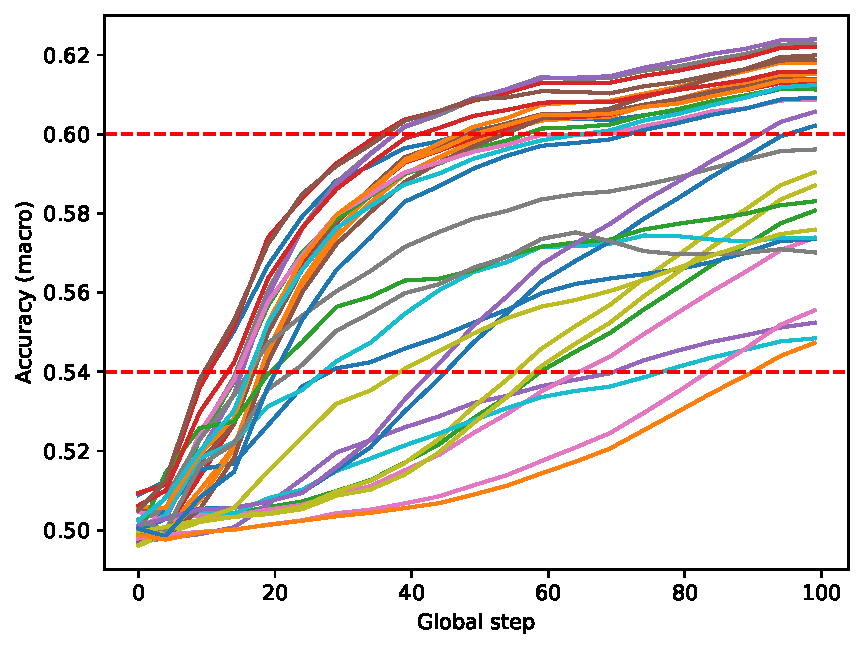
\includegraphics[width=\linewidth]{img/lr.pdf}
    \caption{Convergence processes of 32 models using LSTM+CNN as feature extractor.}
    \label{fig:lr}
\end{figure}

\vspace{2mm}

% tôi có thể viết thêm 1 phần phụ lục nhằm phân tích tác động của lookback window
% Tuy vậy, quá trình hội tụ của chúng tôi lại phụ thuộc rất lớn vào lookback window. Thử nghiệm trên mô hình \verb|LSTM| với dữ liệu \verb|NHITS| cho thấy, khi xét trên cùng một tập siêu tham số và cùng một kiến trúc mô hình, nếu tăng lookback window từ 10 lên 20, số lượng mô hình hội tụ tăng đột biến. Ngoài ra, mức hội tụ mô hình cũng được cải thiện đáng kể. Khi tăng lookback window từ 20 lên 30, xuất hiện một số mô hình tiềm năng, mà độ chính xác của những mô hình này có thể tiếp tục tăng nếu tiếp tục huấn luyện. Đây là một insight thú vị cho thấy nếu nhìn vào quá khứ đủ nhiều và đủ sâu, chúng ta có thể tăng độ chính xác trong các dự đoán tương lai. Nếu dữ liệu quá khứ nhiều hơn, có thể sẽ phải tăng kích thước mô hình để đáp ứng việc hiểu được dữ liệu này.

However, the convergence process of the proposed method depends heavily on the lookback window. Experiments on the \verb|LSTM| model with \verb|NHITS| data show that, when considering the same set of hyper-parameters and the same model architecture, if the lookback window is increased from 10 to 20, the number of converged models increases dramatically. In addition, the model convergence level is also significantly improved. When increasing the lookback window from 20 to 30, some potential models appear, the accuracy of which can continue to increase if training continues. This is an interesting insight showing that if we look into the past enough and deeply enough, we can increase the accuracy in future predictions. If the past data is larger, we may have to increase the model size to meet the understanding of this data.

\begin{figure}[H]
    \centering
    \begin{subfigure}[b]{\linewidth}
        \centering
        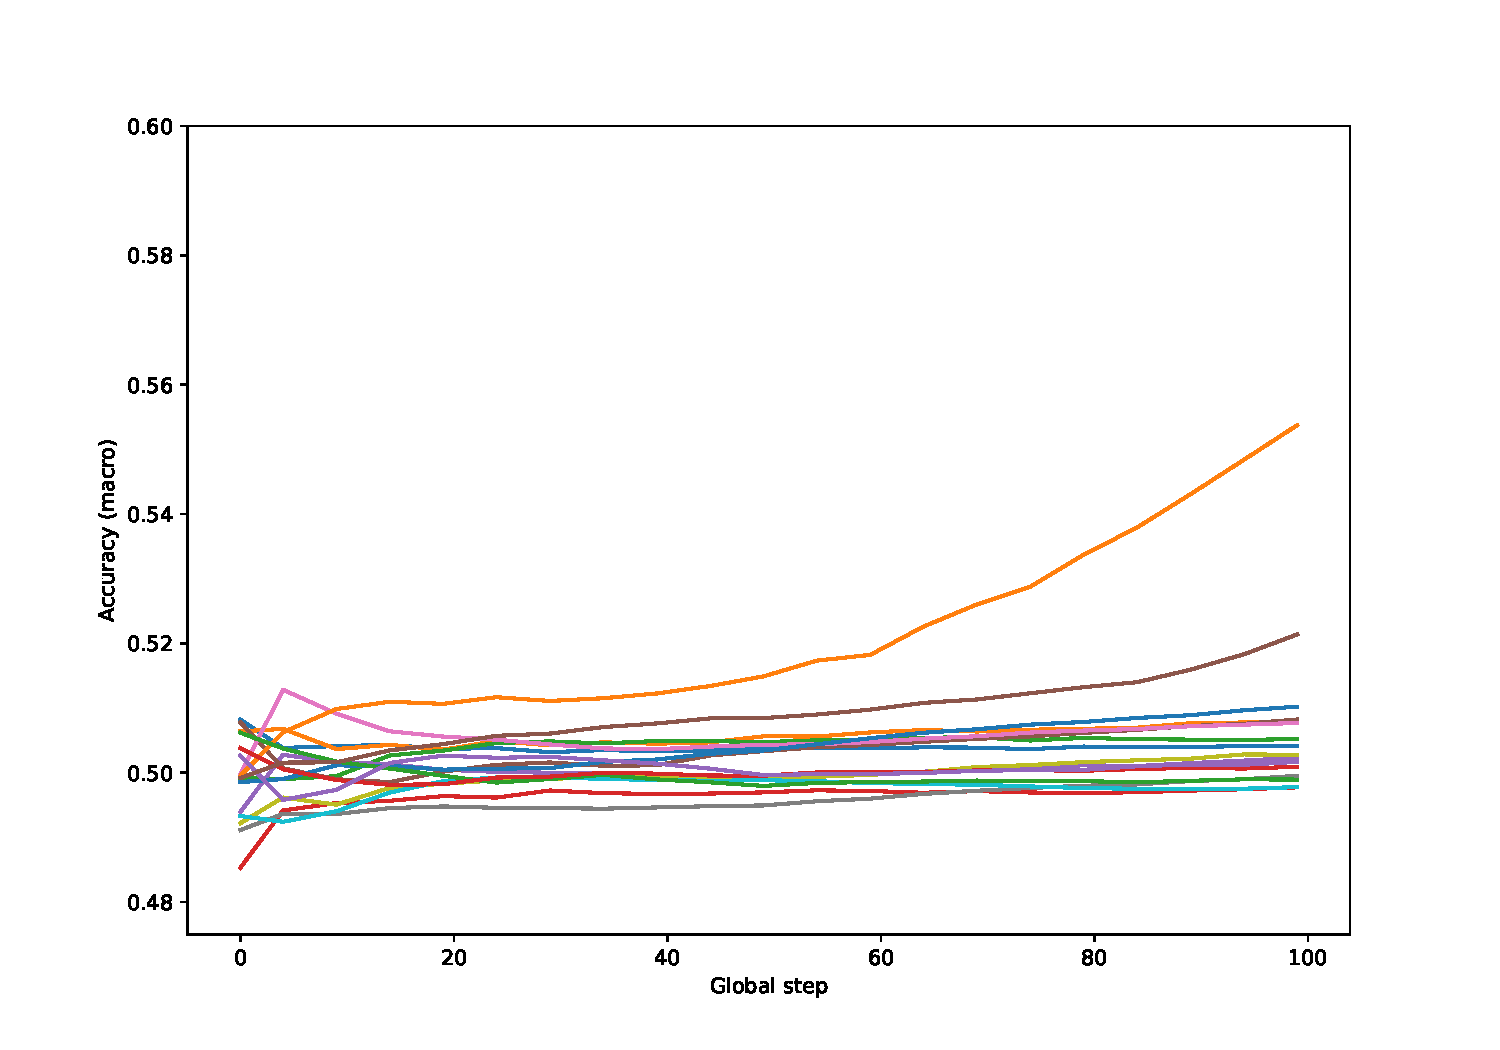
\includegraphics[width=\textwidth]{img/lstm_10.pdf}
        \caption{lookback window = 10}
        \label{fig:image1}
    \end{subfigure}
    % \hfill
    % \vspace{2mm}
    \begin{subfigure}[b]{\linewidth}
        \centering
        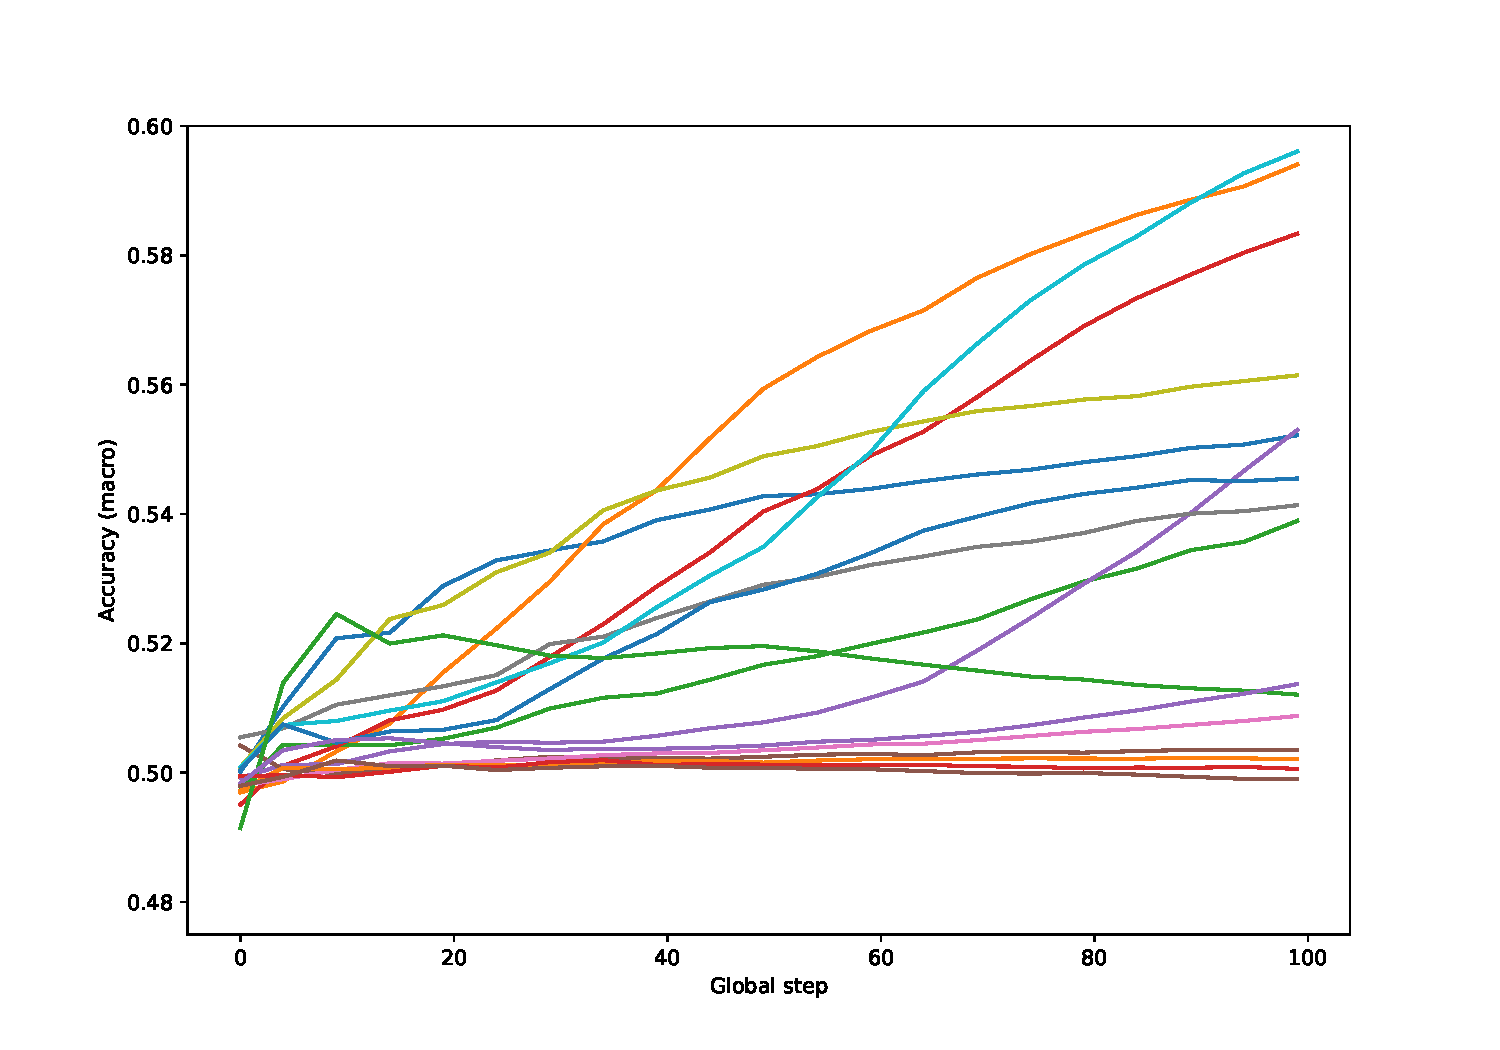
\includegraphics[width=\textwidth]{img/lstm_20.pdf}
        \caption{lookback window = 20}
        \label{fig:image2}
    \end{subfigure}
    % \hfill
    % \vspace{2mm}
    \begin{subfigure}[b]{\linewidth}
        \centering
        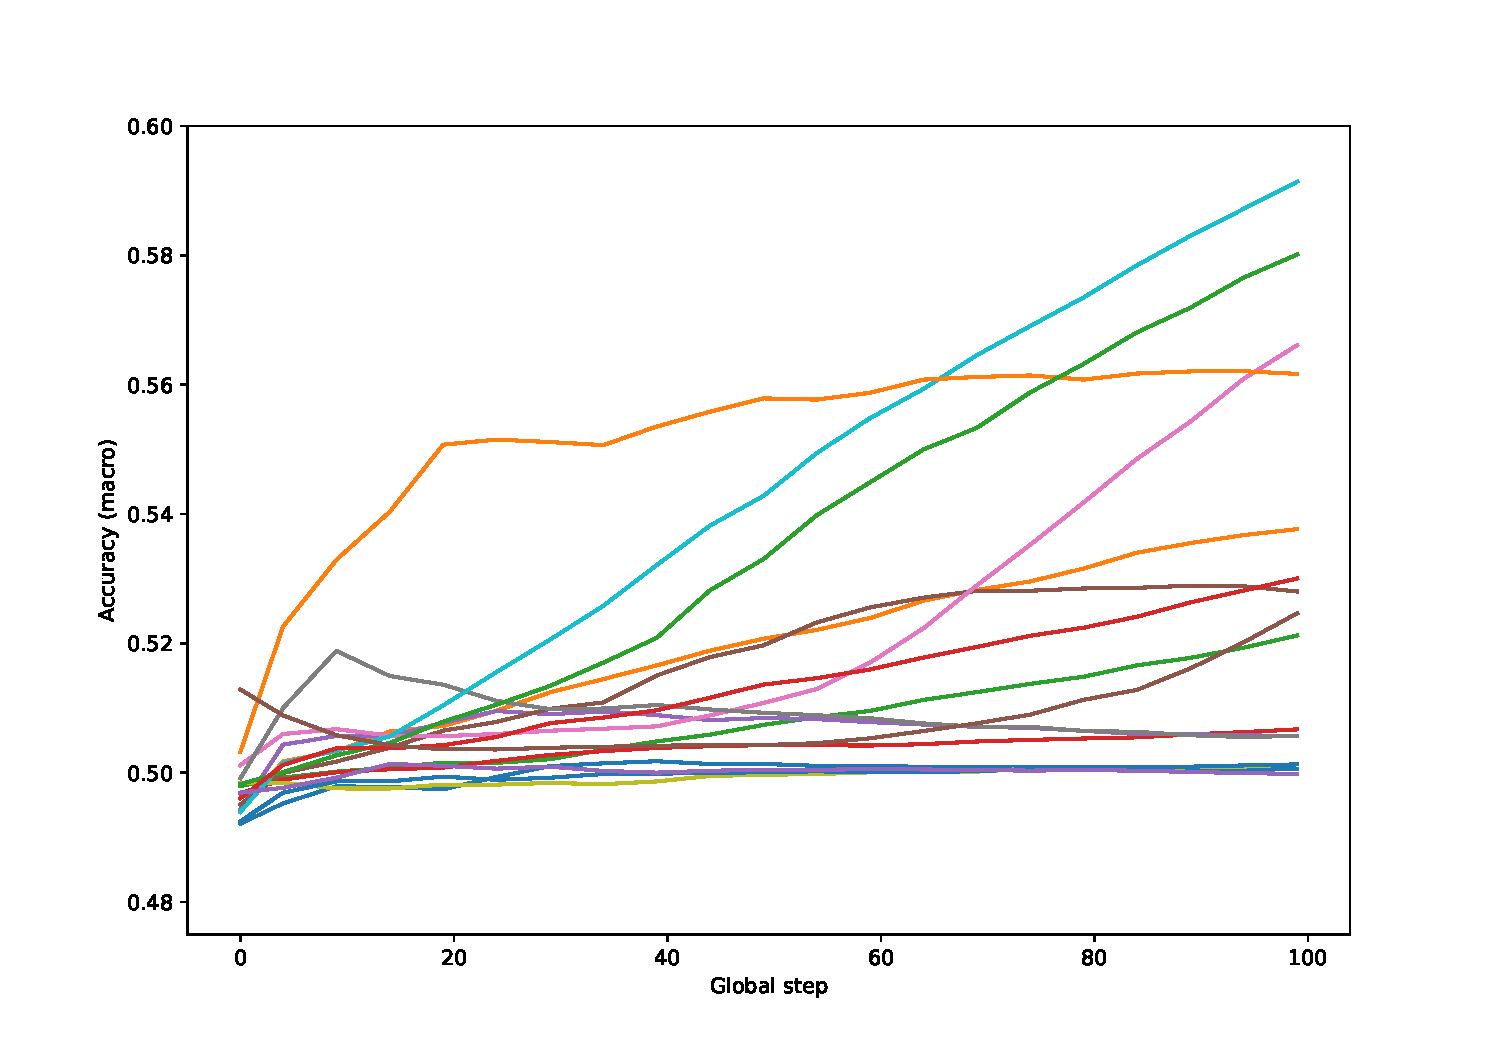
\includegraphics[width=\textwidth]{img/lstm_30.pdf}
        \caption{lookback window = 30}
        \label{fig:image3}
    \end{subfigure}
    \caption{Change in the model's convergence process when changing the lookback window.}
    \label{fig:three_images}
\end{figure}

\end{document}